% pdflatex cmp.tex && pdflatex cmp.tex && del cmp.out, cmp.toc, cmp.log, cmp.aux && start cmp.pdf
\documentclass[a4paper, 12pt]{article}
\usepackage[T2A,T1]{fontenc}
\usepackage[utf8]{inputenc}
\usepackage[english, ukrainian]{babel}
\usepackage{amsmath, amssymb}
\usepackage{float,multirow,xcolor,hyperref}
\hypersetup{unicode=true,colorlinks=true,linktoc=all,linkcolor=red}
\usepackage{amsthm}
\newtheorem{theorem}{Теорема}
\newtheorem{lemma}{Лема}
\newcommand{\RR}{\mathbb{R}}
\newcommand{\Sum}{\displaystyle\sum\limits}
\newcommand{\Prod}{\displaystyle\prod\limits}
\DeclareMathOperator*{\argmax}{arg\,max}
\DeclareMathOperator*{\argmin}{arg\,min}
\DeclareMathOperator{\trace}{tr}
\DeclareMathOperator{\rang}{rang}
\allowdisplaybreaks
\setlength\parindent{0pt}
\title{{\Huge АНАЛІЗ ДАНИХ}}
\author{Нікіта Скибицький}
\date{\today}
\begin{document}
\maketitle \thispagestyle{empty} \newpage 
У ваших руках конспект лекцій з нормативного курсу ``Вступ до аналізу даних'', прочитаного доц., к.ф.-м.н. Слабоспицьким Олександром Сергійовичем на третьому курсі спеціальності прикладна математика факультету комп'ютерних наук та кібернетики Київського національного університету імені Тараса Шевченка восени 2018-го року. \\

Конспект у компактній формі відображає матеріал курсу, допомагає сформувати загальне уявлення про предмет вивчення, правильно зорієнтуватися в даній галузі знань. Конспект лекцій з названої дисципліни сприятиме більш успішному вивченню дисципліни, причому більшою мірою для студентів заочної форми, екстернату, дистанційного та індивідуального навчання. \\

Комп'ютерний набір та верстка -- Скибицький Нікіта Максимович. \newpage
\tableofcontents \newpage
\section{Аналіз похибок заокруглення}

\subsection{Види похибок}

Нехай необхідно розв’язати рівняння
\begin{equation}
	\label{eq:1.1}
	Au = f.
\end{equation}
За рахунок неточно заданих вхідних даних насправді ми маємо рівняння
\begin{equation}
	\label{eq:1.2}
	\tilde A \tilde u = \tilde f.
\end{equation}
Назвемо $\delta_1 = u - \tilde u$ -- \textit{неусувною похибкою}. \\

Застосування методу розв‘язання \eqref{eq:1.2} приводить до рівняння
\begin{equation}
	\label{eq:1.3}
	\tilde A_h \tilde u_h = \tilde f_h,
\end{equation}
де $h > 0$ -- малий параметр. Назвемо $\delta_2 \tilde u - \tilde u_h$ -- \textit{похибкою методу}. \\

Реалізація методу на ЕОМ приводить до рівняння
\begin{equation}
	\label{eq:1.4}
	\tilde A_h^* \tilde u_h^* = \tilde f_h^*.
\end{equation}
Назвемо $\delta_3 = \tilde u_h^* - \tilde u_h$ -- \textit{похибкою заокруглення}. \\

Тоді \textit{повна похибка} $\delta = u - \tilde u_h^* = \delta_1 + \delta_2 + \delta_3$. \\

\begin{definition}
	Кажуть, що задача \eqref{eq:1.1} \textit{коректна}, якщо
	\begin{enumerate}
		\item $\forall f \in F$ $\exists! u \in U$;
		\item задача \eqref{eq:1.1} \textit{стійка}, тобто
		\begin{equation}
			\label{eq:1.5}
			\forall \epsilon > 0 \quad \exists \delta > 0: \|A-\tilde A\| < \delta, \|f-\tilde f\| < \delta \Rightarrow \|u - \tilde u\| < \epsilon.
		\end{equation}
	\end{enumerate}
\end{definition}

Якщо задача \eqref{eq:1.1} \textit{некоректна}, то або розв‘язок її не існує, або він неєдиний, або він нестійкий, тобто 
\begin{equation}
	\label{eq:1.6}
	\exists \epsilon > 0: \forall \delta > 0: \exists A, f: \| A - \tilde A\|<\delta, \|f-\tilde f\| < \delta, \|u-\tilde u\| > \epsilon.
\end{equation}

\textit{Абсолютна похибка} $\Delta (x^*) \ge \max_x |x - x^*|$. \\

\textit{Відносна похибка} $\delta (x^*) \ge \max_x \Delta (x^*) / |x^*|$. \\

\textit{Значущими цифрами} називаються всі цифри, починаючи з першої ненульової зліва. \\

\textit{Вірна цифра} -- це значуща, якщо абсолютна похибка за рахунок відкидання всіх молодших розрядів не перевищує одиниці розряду цієї цифри. Тобто, якщо 
\begin{equation}
	\label{eq:1.7}
	x^* = \overline{\alpha_n \ldots \alpha_0.\alpha_{-1}\ldots\alpha_{-p}\ldots},
\end{equation}
то $\alpha_{-p}$ -- вірна, якщо $\Delta (x^*) \le 10^{-p}$. \\

Інколи $\Delta (x^*) \le w \cdot 10^{-p}$, $1/2 \le w < 1$, наприклад, $w = 0.55$.

\subsection{Підрахунок похибок в ЕОМ}

Підрахуємо відносну похибку заокруглення числа $x$ на ЕОМ з плаваючою комою. В $\beta$-ічній системі числення число представляється у вигляді
\begin{equation}
	\label{eq:1.8}
	x = \pm (\alpha_1 \beta^{-1} + \alpha_2 \beta^{-2} + \ldots + \alpha_t \beta^{-t} + \ldots) \beta^p,
\end{equation}
де $0 \le \alpha_k < \beta$, $\alpha_1 \ne 0$, $k = 1,2,\ldots$ \\

Якщо в ЕОМ $t$ розрядів, то при відкиданні молодших розрядів ми оперуємо з наближеним значенням 
\begin{equation}
	\label{eq:1.9}
	x^* = \pm (\alpha_1 \beta^{-1} + \alpha_2 \beta^{-2} + \ldots + \alpha_t \beta^{-t}) \beta^p,
\end{equation}
і відповідно похибка заокруглення 
\begin{equation}
	\label{eq:1.9_1}
	x - x^* = \pm \beta^p (\alpha_{t+1} \beta^{-t-1} + \ldots)
\end{equation}
Тоді її можна оцінити так
\begin{multline}
	\label{eq:1.10}
	|x - x^*| \le \beta^{p-t-1} \cdot (\beta-1) \cdot (1 + \beta^{-1}+\ldots)\le\\
	\le \beta^{p-t-1} \cdot (\beta-1) \cdot \dfrac{1}{1-\beta^{-1}}=\beta^{p-t}.
\end{multline}

Якщо в представлені \eqref{eq:1.8} взяти $\alpha_1 = 1$, то $|x| \ge \beta^p \cdot \beta^{-1}$. Звідси остаточно 
\begin{equation}
	\label{eq:1.11}
	\delta (x^*) \le \dfrac{\beta^{p-t}}{\beta^{p-1}}=\beta^{1-t}.
\end{equation}

При більш точних способах заокруглення можна отримати оцінку $\delta (x^*) \le \beta^{1-t} / 2 = \epsilon$. Число $\epsilon$ називається ``машинним іпсилон''. Наприклад, для $\beta = 2$, $t = 24$, $\epsilon = 2^{-24} \approx 10^{-7}$.

\subsection{Підрахунок похибок обчислення значення функції}

Нехай задана функція 
\begin{equation}
	\label{eq:1.11_1}
	y = f(x_1, \ldots, x_n) \in C^1(\Omega)
\end{equation}
Необхідно обчислити її значення при наближеному значенні аргументів 
\begin{equation}
	\label{eq:1.11_2}
	\vec x^* = (x_1^*, \ldots, x_n^*),
\end{equation}
де $|x_i - x_i^*| \le \Delta (x_i^*)$ та оцінити похибку обчислення значення функції
\begin{equation}
	\label{eq:1.11_3}
	y^* = f(x_1^*, \ldots, x_n^*).
\end{equation}

Маємо 
\begin{equation}
	\label{eq:1.12}
	|y-y^*| = |f\left(\vec x\right) - f\left(\vec x^*\right)| = \left| \Sum_{i=1}^n \dfrac{\partial f}{\partial x_i} \left(\vec \xi\right) (x_i - x_i^*) \right| \le \Sum_{i=1}^n B_i \cdot \Delta (x_i^*), 
\end{equation}
де 
\begin{equation}
	\label{eq:1.13}
	B_i = \Max_{\vec x \in U} \left| \dfrac{\partial f}{\partial x_i}\left(\vec x\right) \right|.
\end{equation}

Тут 
\begin{equation}
	\label{eq:1.14}
	U = \left\{ \vec x = (x_1, \ldots, x_n): |x_i - x_i^*| \le \Delta (x_i^*)\right\} \in \Omega, \quad i=\overline{1,n}.
\end{equation}
Отже
\begin{equation}
	\label{eq:1.15}
	\Delta (y^*) = |y - y^*| \prec \Sum_{i=1}^n n_i \cdot \Delta (x_i^*),
\end{equation}
з точністю до величин першого порядку малості по
\begin{equation}
	\label{eq:1.15_1}
	\Delta (x^*) = \Max_{i=\overline{1,n}} \Delta (x_i^*),
\end{equation}
де
\begin{equation}
	\label{eq:1.16}
	b_i = \left| \dfrac{\partial f}{\partial x_i}\left(\vec x^*\right) \right|
\end{equation}
та ``$\prec$'' означає приблизно менше. \\

\subsubsection{Похибки арифметичних операцій}

\begin{enumerate}
	\item Сума: $y = x_1 + x_2$, $x_1, x_2 > 0$, 
	\begin{equation}
		\label{eq:1.17}
		\begin{aligned}
		\Delta (y^*) &\le \Delta (x_1^*) + \Delta (x_2^*), \\ 
		\delta (y^*) &\le \dfrac{\Delta (x_1^*) + \Delta (x_2^*)}{x_1^* + x_2^*} \le \max\{\delta (x_1^*), \delta (x_2^*)\}.
		\end{aligned}
	\end{equation}
	
	\item Різниця: $y = x_1 - x_2$, $x_1 > x_2 > 0$,
	\begin{equation}
		\label{eq:1.18}
		\begin{aligned}
		\Delta (y^*) &\le \Delta (x_1^*) + \Delta (x_2^*), \\
		\delta (y^*) &\le \dfrac{x_2^* \delta (x_1^*) + (x_1^*) \delta (x_2^*)}{x_1^* - x_2^*}.
		\end{aligned}
	\end{equation}
	
	При близьких $x_1^*$, $x_2^*$ зростає відносна похибка (за рахунок втрати вірних цифр).

	\item Добуток: $y = x_1 \cdot x_2$, $x_1, x_2 > 0$,
	\begin{equation}
		\label{eq:1.19}
		\begin{aligned}
		\Delta (y^*) &\prec x_2^* \Delta (x_1^*) + x_1^* \Delta (x_2^*), \\
		\delta (y^*) &\le \delta (x_1^*) + \delta (x_2^*).
		\end{aligned}
	\end{equation}

	\item Частка: $y = \dfrac{x_1}{x_2}$, $x_1, x_2 > 0$,
	\begin{equation}
		\label{eq:1.20}
		\begin{aligned}
		\Delta (y^*) &\prec \dfrac{x_2^* \Delta (x_1^*) + x_1^* \Delta (x_2^*)}{(x_2^*)^2}, \\
		\delta (y^*) &\le \delta (x_1^*) + \delta (x_2^*).
		\end{aligned}
	\end{equation}

	При малих $x_2^*$ зростає абсолютна похибка (за рахунок зростання результату ділення). 
\end{enumerate}

\subsection{Обернена задача аналізу позибок}

Нагадаємо, що \textit{пряма задача} аналізу похибок полягає у обчисленні $\Delta (y^*), \delta (y^*)$ по заданих $\Delta (x_i^*)$, $i = \overline{1, n}$. \\

\textit{Обернена задача} полягає у знаходженні $\Delta (x_i^*)$, $i = \overline{1, n}$ по заданих $\Delta (y^*)$, $\delta (y^*)$. Якщо $n > 1$, маємо одну умову 
\begin{equation}
	\label{eq:1.21}
	\Sum_{i=1}^n b_i \Delta (x_i^*) < \epsilon
\end{equation}
для багатьох невідомих $\Delta (x_i^*)$. Вибирають їх із однієї з умов 
\begin{equation}
	\label{eq:1.22}
	b_i \Delta (x_i^*) < \dfrac{\epsilon}{n},
\end{equation}
або
\begin{equation}
	\label{eq:1.23}
	\Delta (x_i^*) < \dfrac{\epsilon}{\Sum_{i=1}^n b_i}.
\end{equation}
\section{Нелінійні рівняння}

\textit{Постановка задачі}. Нехай маємо рівняння $f(x) = 0$, $\overline{x}$ -- його розв’язок, тобто $f (\overline{x}) \equiv 0$. \\

Задача розв‘язання цього рівняння розпадається на етапи:
\begin{enumerate}
	\item Існування та кількість коренів.
	\item Відділення коренів, тобто розбиття числової вісі на інтервали, де знаходиться один корінь.
	\item Обчислення кореня із заданою точністю $\epsilon$.
\end{enumerate}

Для розв'язання перших двох задач використовуються методи математичного аналізу та алгебри, а також графічний метод. Далі розглядаються методи розв'язання третього етапу.

\subsection{Метод ділення навпіл}

Припустимо на $[a, b]$ знаходиться лише один корінь рівняння 
\begin{equation}
	\label{eq:2.1}
	f(x) = 0,
\end{equation}
для $f(x) \in C([a,b])$, який необхідно визначити. Нехай $f(a) \cdot f (b) < 0$. \\

Припустимо, що $f(a) > 0$, $f(b) < 0$. Покладемо $x_1 = \frac{a + b}{2}$ і підрахуємо
$f(x_1)$. Якщо $f_1(x) < 0$, тоді шуканий корінь $x$ знаходиться на інтервалі $(a, x_1)$. Якщо ж $f_1(x) > 0$, то $\overline{x} \in (x_1, b)$, тобто з двох інтервалів $(a, x_1)$ і $(x_1, b)$ вибираємо той, на границях якого функція $f(x)$ має різні знаки, знаходимо точку $x_2$ -- середину вибраного інтервалу, підраховуємо $f(x_2)$ і повторюємо вказаний процес. \\

В результаті отримаємо послідовність інтервалів, що містять шуканий корінь $\overline{x}$, причому довжина кожного послідуючого інтервалу вдвічі менше попереднього. \\

Цей процес продовжується до тих пір, поки довжина отриманого інтервалу $(a_n, b_n)$ не стане меншою за $b_n - a_n < 2 \epsilon$. Тоді $x_{n+1}$, як середина інтервалу $(a_n, b_n)$ пов'язане з $\overline{x}$ нерівністю
\begin{equation}
	\label{eq:2.2}
	|x_n+1 - \overline{x}| < \epsilon.
\end{equation}

Ця умова для деякого $n$ буде виконуватись за теоремою Больцано-Коші. \\

Оскільки
\[ |b_{k + 1} - a_{k + 1} | = \dfrac12 |b_k - a_k|, \]
то
\begin{equation}
	\label{eq:2.3}
	|x_{n+1} - \overline{x}| \le \dfrac{1}{2^{n+1}} (b - a) < \epsilon.
\end{equation}

Звідси отримаємо нерівність для обчислення кількості ітерацій $n$ для виконання умови (\ref{eq:2.2}):
\[ n = n(\epsilon) \ge \left\lfloor \log\left(\dfrac{b-a}{\epsilon}\right) \right\rfloor + 1. \]

Степінь збіжності -- лінійна, тобто геометричної прогресії з знаменником $q = \frac12$. \\

Переваги методу: простота, надійність. Недоліки методу: низька швидкість збіжності; метод не узагальнюється на системи. 

\subsection{Метод простої ітерації}

Спочатку рівняння
\begin{equation}
	\label{eq:2.4}
	f (x) = 0
\end{equation}
замінюється еквівалентним
\begin{equation}
	\label{eq:2.5}
	x = \phi(x)
\end{equation}
Ітераційний процес має вигляді
\begin{equation}
	\label{eq:2.6}
	x_{n+1} = \phi(x_n), \quad n = 0,1,\ldots
\end{equation}

Початкове наближення $x_0$ задається. \\

Для збіжності велике значення має вибір функції $\phi(x)$. Перший спосіб заміни рівняння полягає в відділенні змінної з якогось члена рівняння. Більш продуктивним є перехід від рівняння (\ref{eq:2.4}) до (\ref{eq:2.5}) з функцією $\phi (x) = x + \tau (x) \cdot f (x)$, де $\tau (x)$ -- знакостала функція на тому відрізку, де шукаємо корінь. \\

Кажуть, що ітераційний метод \textit{збігається}, якщо $\Lim_{k\to\infty} x_k = \overline{x}$. \\

Далі $U_r = \{x : |x - a| \le r\}$ відрізок довжини $2r$ з серединою в точці $a$. \\

З'ясуємо умови, при яких збігається метод простої ітерації.

\begin{theorem}
	Якщо $\Max_{x \in U_r} |\phi'(x)| \le q < 1$, то метод простої ітерації збігається і має місце оцінка 
	\begin{equation}
		\label{eq:2.7}
		|x_n - \overline{x}| \le \dfrac{q^n}{1-q}|x_0-x_1| \le \dfrac{q^n}{1-q}(b-a).
	\end{equation}
\end{theorem}

\begin{proof}
	Нехай $x_{k+1}, x_k \in U_r$. Тоді має місце допоміжна нерівність:
	\begin{multline*}
		|x_{k+1} - x_k| = |\phi(x_k) - \phi(x_{k-1})| = |\phi'(\xi_k)(x_k - x_{k-1}) \le (*) \\
		\text{тут }\xi_k = x_k + \theta_k (x_{k+1} - x_k), \quad 0 < \theta_k < 1 \\
		(*) \le |\phi'(\xi_k)| \cdot |x_k - x_{k-1}| \le q |x_k - x_{k-1}| = \ldots = q^k |x_1 - x_0|.
	\end{multline*}
	Використаємо її для доведення теореми:
	\begin{multline}
		\label{eq:2.8}
		|x_{k+p} - x_k| = |x_{k+p} - x_{k+p-1} + \ldots + x_{k+1} - x_k| \le \\
		\le |x_{k+p} - x_{k+p-1}| + \ldots + |x_{k+1} - x_k| \le \\
		\le (q^{k+p-1}+q^{k+p-2}+\ldots+q^k) |x_1 - x_0| = \\
		= \dfrac{q^k - q^{k+p-1}}{1-q}|x_1-x_0| \xrightarrow[k\to\infty]{}0.
	\end{multline}

	Бачимо що $\{x_k\}$ -- фундаментальна послідовність. Значить вона збіжна. При $p\to\infty$ в (\ref{eq:2.8}) отримуємо (\ref{eq:2.7}).
\end{proof}

Визначимо кількість ітерацій для досягнення точності $\epsilon$. З оцінки в теоремі отримаємо \[ |x_n - \overline{x}| \le \dfrac{q^n}{1-q}(b-a) < \epsilon \Rightarrow n(\epsilon) = n \ge \left\lfloor \dfrac{\ln \left(\dfrac{\epsilon (1-q)}{b - a}\right)}{\ln q} \right\rfloor + 1. \]

Практично ітераційний процес зупиняємо при: $|x_n - x_{n-1}| < \epsilon$. Але ця умова не завжди гарантує, що $|x_n - \overline{x}| < \epsilon$.

\begin{remark*}
	Умова збіжності методу може бути замінена на умову Ліпшиця \[|\phi(x) -\phi(y)| \le q \cdot| x - y |,\quad 0 < q < 1.\]
\end{remark*}

Переваги методу: простота; при $q < \frac12$ -- швидше збігається ніж метод ділення навпіл; метод узагальнюється на системи. Недоліки методу: 
\begin{enumerate}
	\item при $q > \frac12$ -- збігається повільніше ніж метод ділення навпіл,
	\item виникають труднощі при зведенні $f (x) = 0$ до $x =\phi (x)$.
\end{enumerate}


\subsection{Метод релаксації}

Якщо в методі простої ітерації для рівняння $x = x +\tau f (x) \equiv\phi (x)$ вибрати $\tau (x) =\tau = \const$, то ітераційний процес приймає вигляд
\begin{equation}
	\label{eq:2.9}
	x_{n+1} = x_n +\tau \cdot f(x_n), \quad n = 0,1,2,\ldots
\end{equation}
$x_0$ -- задано. Метод можна записати у вигляді \[\dfrac{x_{k+1}-x_k}{\tau} = f(x_k), \quad k=0,1,\ldots.\] Оскільки $\phi'(x) =1+\tau\cdot f'(x)$, то метод збігається при умові \[ |\phi'(x)| = |1+\tau \cdot f'(x)| \le q < 1.\]

Нехай $f'(x) < 0$, тоді (\ref{eq:2.7}) запишеться у вигляді: $-q \le 1 +\tau \cdot f'(x) \le q < 1$. Звідси \[\tau \cdot |f'(x_k)| \le 1 + q < 2 \quad \text{і} \quad 0 < \tau < \dfrac{2}{|f'(x)|}. \]

Поставимо задачу знаходження $\tau$, для якого $q = q(\tau) \to \min$. Для того, щоб вибрати оптимальний параметр $\tau$, розглянемо рівняння для похибки $z_k = x_j - \overline{x}$. \\

Підставивши $x_k = x + z_k$ в (\ref{eq:2.9}), отримаємо
\[ z_{k+1} = z_k + \tau \cdot f(\overline{x} + z_k).\]

В припущені $f(x)\in C^{(1)}([a,b])$ з теореми про середнє маємо
\[ f(\overline{x} + z_k) = f(\overline{x}) + z_k \cdot f'(\overline{x} + \theta z_k) = z_k \cdot f'(\overline{x}+\theta z_k) = z_k \cdot f'(\xi_k), \]
\[ z_{k+1} = z_k + \tau \cdot f'(\xi_k) \cdot z_k, \]
\[ |z_{k+1}| \le |1 + \tau \cdot f'(\xi_k)| \cdot |z_k| \le \Max_{\xi_k \in U} |1 + \tau \cdot f'(\xi_k)| \cdot |z_k|, \]
\[ |z_{k+1}| \le \max \{|1-\tau \cdot M_1|, |1-\tau \cdot m_1| \}\cdot |z_k|, \]
\[ m_1 = \Min_{x\in[a,b]} |f'(x)|, \quad M_1 = \Max_{x\in[a,b]} |f'(x)|. \]

Таким чином, задача вибору оптимального параметра зводиться до знаходження $\tau$, для якого функція \[ q(\tau) = \max\{|1-\tau \cdot M_1|,|1-\tau \cdot m_1|\}\]
приймає мінімальне значення: $q(\tau)\to\min$.

\begin{figure}[H]
	\centering
	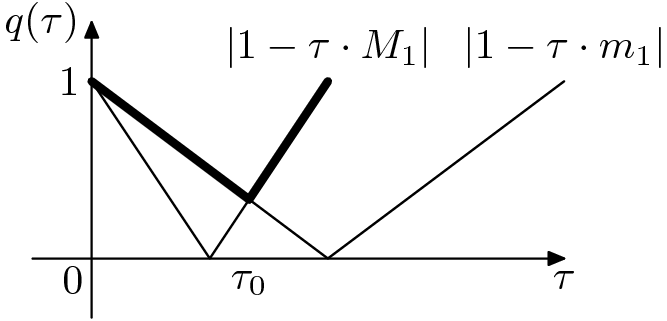
\includegraphics[width=.5\linewidth]{mal-1.png}
\end{figure}

% u:=1cm;
% label.llft(btex $0$ etex, (0,0));
% label.lft(btex $1$ etex, (0,3u/2));
% drawarrow (-u/2,0)--(4u,0);
% drawarrow (0,-u/2)--(0,2u);
% label.lft(btex $q(\tau)$ etex, (0,2u));
% label.bot(btex $\tau$ etex, (4u,0));
% draw (0,3u/2)--(u,0)--(2u,3u/2);
% draw (0,3u/2)--(2u,0)--(4u,3u/2);
% label.top(btex $|1-\tau \cdot M_1|$ etex, (2u,3u/2));
% label.top(btex $|1-\tau \cdot m_1|$ etex, (4u,3u/2));
% draw (4/3u,u/2)--(2u,3u/2) withpen pencircle scaled 2bp;
% draw (0,3u/2)--(4/3u,u/2) withpen pencircle scaled 2bp;
% label.bot(btex $\tau_0$ etex, (4/3u,0));

З графіка видно, що точка мінімуму визначається умовою $|1 - \tau \cdot M_1| = |1 - \tau \cdot m_1|$. \\

Тому
\[ 1 - \tau_0 \cdot m_1 = \tau_0 \cdot M_1 - 1 \Rightarrow \tau_0 = \dfrac{2}{M_1+m_1} < \dfrac{2}{|f'(x)|}.\]

При цьому значенні $\tau$ маємо \[q(\tau_0) = q_0 =\dfrac{M_1-m_1}{M_1+m_1}.\]

Тоді для похибки вірна оцінка \[|x_n-\overline{x}|\le \dfrac{q_0^n\cdot (b-a)}{1-q_0}<\epsilon.\]

Кількість ітерацій \[n = n(\epsilon) \ge \left\lfloor \dfrac{\ln \left(\dfrac{\epsilon\cdot(1-q_0)}{b-a}\right)}{\ln q_0} \right\rfloor + 1.\]	

\begin{problem} 
	Дати геометричну інтерпретацію методу простої ітерації для випадків:
	\[ 0 < \phi'(x) < 1; \quad -1 < \phi'(x) < 0; \quad \phi'(x) < -1; \quad \phi'(x) > 1,\]
\end{problem}

\begin{problem} 
	Знайти оптимальне $\tau = \tau_0$ для методу релаксації при $f'(x) > 0$.
\end{problem}

\subsection{Метод Ньютона (метод дотичних)}

Припустимо, що рівняння $f (x) = 0$ має простий дійсний корінь $\overline{x}$, тобто $f (\overline{x}) = 0$, $f'(\overline{x}) \ne 0$. Нехай виконуються умови: $f (x)\in C^{(1)}([a,b])$, $f (a)\cdot f (b) < 0$. Тоді 
\[0 = f (\overline{x}) = f (x_k + \overline{x} - x_k ) = f (x_k ) + f'(\xi_k ) \cdot (\overline{x} - x_k ),\] 
де $\xi_k=x_k+\theta_k \cdot (\overline{x}-x_k)$, $0 < \theta_k < 1$, $\xi_k \approx x_k$. Тому наступне наближення виберемо з рівняння 
\[ f(x_k) + f'(x_k) \cdot (x_{k+1}-x_k) = 0.\]

Звідси маємо ітераційний процес
\[ x_{k+1} = x_k - \dfrac{f(x_k)}{f'(x_k)}, \quad k = 0,1,2,\ldots, \quad x_0\text{ -- задане}. \]

Метод Ньютона ще називають методом лінеаризації або методом дотичних.

\begin{problem} 
	Дати геометричну інтерпретацію методу Ньютона.
\end{problem}

Метод Ньютона можна інтерпретувати як метод простої ітерації з \[ \phi(x) = x - \dfrac{f(x)}{f'(x)}, \quad \text{тобто} \quad \tau(x) = - \dfrac{1}{f'(x)}. \]

Тому 
\[ \phi'(x) = 1 - \dfrac{f'(x)\cdot f'(x)-f(x)\cdot f''(x)}{(f'(x))^2} = \dfrac{f(x)\cdot f''(x)}{(f'(x))^2}.\]
Якщо $\overline{x}$ -- корінь $f(x)$, то $\phi'(x) = 0$. Тому знайдеться окіл кореня, де \[ |\phi'(x)| = \left|\dfrac{f(x)\cdot f''(x)}{(f'(x))^2}\right|<1.\]

Це означає, що збіжність методу Ньютона залежить від вибору $x_0$. \\

Недолік методу Ньютона: необхідність обчислювати на кожній ітерації не тільки значення функції, а й похідної. \\

Модифікований метод Ньютона позбавлений цього недоліку і має вигляд:
\[ x_{k+1} = x_k - \dfrac{f(x_k)}{f'(x_0)}, \quad k=0,1,2,\ldots. \]

Цей метод має лише лінійну збіжність: $|x_{k+1} - \overline{x}| = O(|x_k-\overline{x}|)$.
\begin{problem} 
	Дати геометричну інтерпретацію модифікованого методу Ньютона.
\end{problem}

В методі Ньютона, для якого $f'(x_k)$ замінюється на $\frac{f(x_k)-f(x_{k-1})}{x_k-x_{k-1}}$ дає метод січних: \[ x_{k+1} = x_k - \dfrac{x_k-x_{k-1}}{f(x_k)-f(x_{k-1})}\cdot f(x_k), \quad k = 1,2,\ldots, \quad x_0,x_1\text{ -- задані}.\]

\begin{problem} 
	Дати геометричну інтерпретацію методу січних.
\end{problem}

\subsection{Збіжність методу Ньютона}

\begin{theorem}
	Нехай $f(x)\in C^{(2)}([a,b])$, $\overline{x}$ -- простий дійсний корінь рівняння
	\begin{equation}
		\label{eq:2.10}
		f (x) = 0
	\end{equation}
	і $f'(x) \ne 0$ при $x\in U_r= \{x: |x -\overline{x}| < r\}$. Якщо
	\begin{equation}
		\label{eq:2.11}
		\dfrac{M_2\cdot|x_0-\overline{x}|}{2m_1} = q < 1
	\end{equation}
	де $m_1 = \Min_{x\in U_r} |f'(x)|$, $M_2 = \Max_{x\in U_r} |f''(x)|$, то для $x_0 \in U_r$ метод Ньютона 
	\begin{equation}
		\label{eq:2.12}
		x_{k+1} = x_k - \dfrac{f(x_k)}{f'(x_k)}
	\end{equation}
	збігається і має місце оцінка
	\begin{equation}
		\label{eq:2.13}
		|x_n - \overline{x}| \le q^{2^n-1} \cdot |x_0 - \overline{x}|.
	\end{equation}
\end{theorem}

\begin{proof}
	З (\ref{eq:2.12}) маємо 
	\begin{equation}
		\label{eq:2.14}
		x_{k+1} - \overline{x} = x_k - \dfrac{f(x_k)}{f'(x_k)} - \overline{x} = \dfrac{(x_k-\overline{x}) \cdot f'(x_k)-f(x_k)}{f'(x_k)} = \dfrac{F(x_k)}{f'(x_k)},
	\end{equation}
	де $F(x) = (x - \overline{x}) \cdot f'(x) - f (x)$, така, що
	\begin{enumerate}
		\item $F(x) = 0$;
		\item $F'(x) = (x - \overline{x}) \cdot f''(x)$;
	\end{enumerate}
	Тоді \[ F(x_k) = F(\overline{x}) + \Int_{\overline{x}}^{x_k}  F'(t) \diff t = \Int_{\overline{x}}^{x_k}  ((t - \overline{x}) \cdot f''(t)) \diff t . \]

	Так як $(t - x)$ не міняє знак на відрізку інтегрування, то скористаємося теоремою про середнє значення:
	\begin{equation}
		\label{eq:2.15}
		F(x_k) = f''(\xi_k) \Int_{\overline{x}}^{x_k}  (t - \overline{x}) \diff t = \dfrac{(x_k-\overline{x})^2}{2} f''(\xi_k),
	\end{equation}
	де $\xi_k = \overline{x} + \theta_k \cdot (x_k - \overline{x})$, $0 <\theta_k < 1$. З (\ref{eq:2.14}), (\ref{eq:2.15}) маємо
	\begin{equation}
		\label{eq:2.16}
		x_{k+1} - \overline{x} = \dfrac{(x_k-\overline{x})^2}{2f'(x_k)} f''(\xi_k).
	\end{equation}
	Доведемо оцінку (\ref{eq:2.12}) за індукцією. Так як $x_0 \in U_r$, то \[|\xi_0 - \overline{x}| = |\theta_0 \cdot (x_0 - \overline{x})| < |\theta_0| \cdot |x_0 - \overline{x}| < r \Rightarrow \xi_0 \in U_r.\]

	Тоді $f''(\xi_0) \le M_2$, тому
	\begin{multline*} 
		|x_1 - \overline{x}| \le \dfrac{(x_0-\overline{x})^2 \cdot M_2}{2m_1} = \dfrac{M_2\cdot|x_0-\overline{x}|}{2m_1}|x_0-\overline{x}| = \\
		= q\cdot |x_0-\overline{x}|=q\cdot |x_0-\overline{x}|<r \Rightarrow x_1\in U_r.
	\end{multline*}

	Ми довели твердження (\ref{eq:2.13}) при $n = 1$. Нехай воно справджується при $n = k$:
	\[ |x_k - \overline{x}| \le q^{2^k-1}\cdot |x_0 - \overline{x}| < r, \quad |\xi_k - \overline{x}| = |\theta_k \cdot (x_k - \overline{x})| < r. \]

	Тоді $x_k, \xi_k \in U_r$. \\

	Доведемо (\ref{eq:2.13}) для $n = k +1$. З (\ref{eq:2.16}) маємо 
	\begin{multline*}
		|x_{k+1}-\overline{x}| \le \dfrac{|x_k - \overline{x}|^2\cdot M_2}{2m_1} \le \left(q^{2^k-1}\right)^2 \dfrac{|x_0-\overline{x}|^2\cdot M_2}{2m_1} = \\
		= q^{2^{k+1}-2} \dfrac{|x_0-\overline{x}|\cdot M_2}{2m_1}|x_0-\overline{x}| = q^{2^{k+1}-1} \cdot |x_0-\overline{x}|.
	\end{multline*}

	Таким чином (\ref{eq:2.13}) справджується для $n = k +1$. Значить (\ref{eq:2.13}) виконується і для довільного $n$. Таким чином $x_n \xrightarrow[n\to\infty]{} \overline{x}$.
\end{proof}

З (\ref{eq:2.13}) маємо оцінку кількості ітерацій для досягнення точності $\epsilon$:
\[ n \ge \left\lfloor\log_2\left(1+\dfrac{\ln \left(\dfrac{\epsilon}{b-a}\right)}{\ln q}\right) \right\rfloor + 1 .\]

Кажуть, що ітераційний метод має \textit{степінь збіжності} $m$, якщо \[ |x_{k+1}-\overline{x}|=O(|x_k-\overline{x}|^m).\]

Для методу Ньютона 
\[|x_{k+1}-\overline{x}| = \dfrac{|x_k-\overline{x}|^2\cdot|f''(\xi_k)|}{2|f'(x_k)|}| \Rightarrow |x_{k+1}-\overline{x}|=O(|x_k-\overline{x}|^2).\]

Значить степінь збіжності методу Ньютона $m=2$. Для методу простої ітерації і ділення навпіл $m=1$.

\begin{theorem}
	Нехай $f(x)\in C^{(2)}([a,b])$ та $\overline{x}$ -- простий корінь рівняння $f (x) = 0$ а також $\forall x\in[a,b]$: $f'(x) \ne 0$. Якщо $f'(x) \cdot f''(x) > 0$ ($f'(x) \cdot f''(x) < 0$) то для методу Ньютона при $x_0 = b$ послідовність наближень $\{x_k \}$ монотонно спадає (монотонно зростає при $x_0 = a$).
\end{theorem}

\begin{problem}
	Довести теорему при 
	\begin{enumerate}
		\item $f'(x) \cdot f''(x) > 0$;
		\item $f'(x) f''(x) < 0$.
	\end{enumerate}
\end{problem}

\begin{problem}
	Знайти степінь збіжності методу січних.
\end{problem}


Якщо $f(a) \cdot f''(a) > 0$ та $f''(x)$ не міняє знак, то потрібно вибирати $x_0 = a$; при цьому $\{x_k \}\uparrow \overline{x}$. \\

Якщо $f(b) \cdot f''(b) > 0$, то $x_0 = b$; маємо $\{x_k \}\downarrow \overline{x}$. Пояснення на рисунку:

% u := 1cm;
% drawarrow (-u/2, 0)--(4u, 0);
% drawarrow (0, -u/2)--(0, 2u);
% draw (u/2,0)--(u/2,u/8);
% draw (7u/2,0)--(7u/2,u/8);
% label.bot(btex $a$ etex, (u/2, 0));
% label.top(btex $b$ etex, (7u/2, u/8));
% draw (u/2,3u/2){dir -75}..(2u,-u/2){dir 0}..(7u/2,-u/4);
% label.top(btex $x_0 = a$ etex, (2u,u));

% u := 1cm;
% drawarrow (-u/2, 0)--(4u, 0);
% drawarrow (0, -u/2)--(0, 2u);
% draw (u/2,0)--(u/2,u/8);
% draw (7u/2,0)--(7u/2,u/8);
% label.top(btex $a$ etex, (u/2, u/8));
% label.bot(btex $b$ etex, (7u/2, 0));
% draw (u/2,-3u/7){dir 75}..(2u,u)..(7u/2,3u/2);
% label.top(btex $x_0 = a$ etex, (2u,3u/2));

\begin{figure}[H]
	\centering
	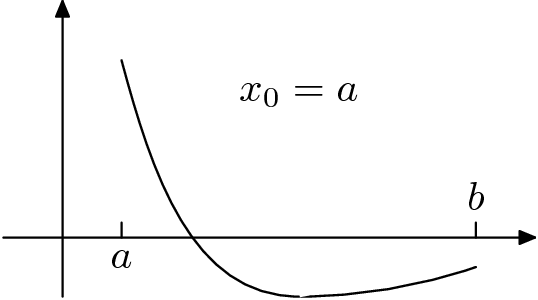
\includegraphics[width=.45\linewidth]{mal-2.png}
	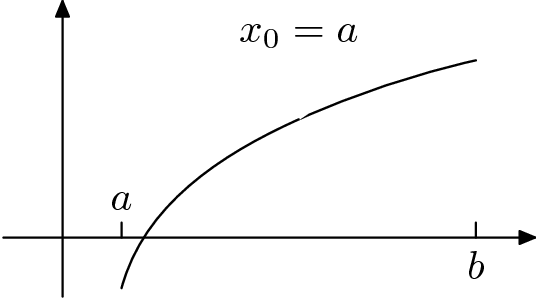
\includegraphics[width=.45\linewidth]{mal-3.png}
\end{figure}

\begin{remark}
	Якщо $\overline{x}$ -- $p$-кратний корінь тобто $f^{(m)} (x) = 0$, $m = \overline{0,p-1}$, $f^{ (p)} (x) \ne 0$, то в методі Ньютона необхідна наступна модифікація \[x_{k+1} = x_k - p\dfrac{f(x_k)}{f'(x_k)} \quad \text{і} \quad q = \dfrac{M_{p+1}\cdot|x_0-\overline{x}|}{m_p \cdot (p+1)}<1.\]
\end{remark}

\begin{remark}
Метод Ньютона можна застосовувати і для обчислення комплексного кореня, тоді ітераційний процес має вигляд \[z_{k+1} = z_k - \dfrac{f(z_k)}{f'(z_k)}, \quad k = 0,1,\ldots.\] В теоремі про збіжність $q = \frac{|z_0-\overline{z}|\cdot M_2}{2m_1}$, де $m_1 = \Min_{z\in U_r} |f'(z)|$, $M_2 = \Max_{z\in U_r} |f''(z)|$. Тут $|z|$ -- модуль комплексного числа $z$.
\end{remark}

Переваги методу Ньютона: 
\begin{enumerate}
\item висока швидкість збіжності;
\item узагальнюється на системи рівнянь; 
\item узагальнюється на комплексні корені.
\end{enumerate}
Недоліки методу Ньютона: 
\begin{enumerate}
	\item на кожній ітерації обчислюється не тільки $f (x_k )$ , а і похідна $f'(x_k)$;
	\item  збіжність залежить від початкового наближення $x_0$, так як від нього залежить умова збіжності $q = \frac{M_2\cdot |x_0-\overline{x}|}{2m_1} < 1$;
	\item потрібно, щоб $f (x)\in C^{(2)}([a,b])$.
\end{enumerate}
\subsubsection{Характеристики розсіювання значень}
Нехай маємо вибірку об'єму $n$ спостережень $x_1$, $x_2$, $\ldots$, $x_n$ над випадковою величиною $\xi$.
\begin{enumerate}
	\item \textit{Дисперсія} $D\xi = M(\xi - M\xi)^2$. Вибіркове значення \[ S^2(n) = \dfrac{1}{n-1} \sum_{i=1}^n (x_i - \bar{x}(n))^2 = \dfrac{1}{n-1} \left(\sum_{i=1}^n x_i^2 - n\bar{x}^2(n) \right). \]
	\item \textit{Стандартне (середньоквадратичне) відхилення} $\sqrt{D\xi}$. Вибіркове значення $S(n)$.
	\item \textit{Коефіцієнт варіацій} $V_\xi = \frac{\sqrt{D\xi}}{M\xi} 100\%$, $M\xi\ne0$. Вибіркове значення $\widehat{V}_\xi(n)=\frac{S(n)}{\bar x(n)} 100\%$.
	\item \textit{Стохастичне розсіювання} (імовірнісне відхилення) -- це половина інтерквартильної широти: $\frac{U_{0.75} - U_{0.25}}{2}$. Вибіркове значення $\frac{\widehat{U}_{0.75} - \widehat{U}_{0.25}}{2}$.
	\item \textit{Розмах (широта) вибірки}: $x_{\max}-x_{\min}$, де $x_{\max}, x_{\min}$ -- найбільше та найменше значення у вибірці.
	\item \textit{Інтервал концентрації} $(M\xi - 3\sqrt{D\xi}, M\xi + 3 \sqrt{D\xi})$. Вибіркове значення $(\bar x(n) - 3S(n), M\bar x(n) + 3 S(n))$.
\end{enumerate}
\subsubsection{Характеристики скошеності та гостроверхості розподілу}
Нехай є розподіл випадкової величини $\xi$ і отримані спостереження $x_1$, $x_2$, $\ldots$, $x_n$ над нею.
\begin{enumerate}
	\item \textit{Коефіцієнт асиметрії} -- характеристика скошеності розподілу (базується на третьому центральному моменті): \[ \beta_1 = \dfrac{M(\xi - M\xi)^3}{(M(\xi - M\xi)^2)^{3/2}}, \quad D\xi > 0. \] Вибіркове значення \[ \widehat{\beta}_1 = \dfrac{\dfrac{1}{n}\Sum_{i=1}^n(x_k - \bar{x}(n))^3}{S^3(n)}. \] Дисперсія спостережуваної величини $D\xi > 0$. \\ % figure 6

	Якщо розподіл симетричний (наприклад нормальний) то $\beta_1 =0$. Якщо $\beta_1 > 0$, то розподіл скошений вліво, якщо $\beta_1 < 0$, то вправо.
	\item \textit{Коефіцієнт ексцесу} -- характеристика гостроверхості розподілу (базується на четвертому центральному моменті): \[ \beta_2 = \dfrac{M(\xi-M\xi)^4}{(M(\xi-M\xi)^2)^2} - 3, \quad D\xi > 0. \] Вибіркове значення \[ \widehat{\beta}_2 = \dfrac{\dfrac{1}{n}\Sum_{i=1}^n(x_k - \bar{x}(n))^4}{S^4(n)} - 3. \]
	Для нормального розподілу коефіцієнт ексцесу дорівнює нулю. Якщо $\beta_2 > 0$, то розподіл більш гостроверхий ніж нормальний, якщо $\beta_2 < 0$ то відповідно менш гостроверхий.
\end{enumerate}
\subsection{Характеристики векторних величин}
Аналіз $q$-вимірних векторних величин, отримано $n$ спостережень над вектором $\vec\xi: x_1, x_2, \ldots, x_n$, $x_i \in \RR^q$, $i = \overline{1,n}$.
\subsubsection{Характеристики положення центру значень}
\begin{enumerate}
	\item \textit{Математичне сподівання} (теоретичне середнє) $M\xi$. Вибіркове значення \[\bar{x}(n) = \dfrac{1}{n} \Sum_{i=1}^n \vec{x}_i.\]
	\item \textit{Мода} $x_{\text{mod}}$. У неперервному випадку -- це точка максимуму функції щільності $\xi$. Для дискретного випадку -- це значення, яке набуває $\xi$ з найбільшою ймовірністю.
\end{enumerate}
\subsubsection{Характеристики розсіювання значень}
\begin{enumerate} 
	\item \textit{Коваріаційна матриця} $\sum = M(\xi - M\xi)(\xi - M\xi)^T$. Вибіркове значення \[\widehat{\sum}(n) = \dfrac{1}{n-1} \Sum_{k=1}^n (x_k - \bar x(n))(x_k - \bar x(n))^T.\]
	\item \textit{Узагальнена дисперсія} -- визначник коваріаційної матриці: $\det \sum$. Вибіркове значення $\det\left(\widehat{\sum}\right)$.
	\item \textit{Слід коваріаційної матриці} $\trace\sum$. Вибіркове значення $\trace\left(\widehat{\sum}(n)\right)$.
\end{enumerate}
\subsection{Перевірка стохастичності вибірки}
Перевіряємо, чи справді вибірка є випадковою, а не знаходиться під впливом деякого систематичного зміщення. Для цього запропоновано критерії:
\begin{itemize}
	\item Критерій серій на базі медіани
	\item Критерій зростаючих та спадаючих серій
	\item Критерій квадратів послідовних різниць (критерій Аббе)
\end{itemize}
Нехай $x_1$, $x_2$, $\ldots$, $x_n$ -- вибірка спостережень, яка досліджується. \\

Будемо перевіряти гіпотезу $H_0$: ця вибірка є стохастичною з рівнем значимості $\alpha (0 < \alpha < 1$) (рівень значимості -- ймовірність допустити помилку першого роду).
\begin{enumerate}
	\item \textit{Критерій серій на базі медіани}. Альтернативна гіпотеза $H_1$: наявність у вибірці систематичного монотонного зміщення середнього. \\

	Спочатку визначається вибіркове значення медіани $\widehat{x}_{\text{med}}$. Потім під кожним членом вибірки ставимо відповідно \[ \begin{cases} +, & x_i > \widehat{x}_{\text{med}} \\
 \text{нічого}, & x_i = \widehat{x}_{\text{med}} \\
 -, & x_i < \widehat{x}_{\text{med}} \end{cases}. \]
	Отримаємо послідовність символів. \textit{Серія} -- послідовність підряд розташованих однакових символів $+$ чи $-$. \textit{Довжина серії} -- це кількість членів у ній. \\

	Для отриманої послідовності обчислюємо дві статистики: загальну кількість серій в послідовності $v(n)$, довжину найдовшої серії $\tau(n)$. Запишемо область прийняття нашої гіпотези: \[ \left\{ \begin{matrix} v(n) > v_\beta(n) \\
 \tau(n) < \tau_{1-\beta}(n) \end{matrix} \right. \] 
	де $v_\beta(n)$, $\tau_\beta(n)$ -- квантилі рівня $\beta$ статистик $v(n)$, $\tau(n)$ відповідно. При фіксованому значенні $\beta$ рівень значимості $\alpha$ лежить у межах $\beta < \alpha < 2\beta - \beta^2$. Якщо порушується хоч одна з нерівностей, то гіпотеза відхиляється.
	\item \textit{Критерій зростаючих та спадаючих серій}. Альтернативна гіпотеза $H_1$: наявність у вибірці систематичного періодичного зміщення середнього. Спочатку у вибірці замінюємо підряд розташовані однакові виміри одним їх представником. В результаті отримаємо послідовність $x_1'$, $x_2'$, $\ldots$, $x_k'$. Під кожним членом послідовності ставимо відповідно \[ \begin{cases} +, & x_i' < x_{i+1}' \\
 -, & x_i' > x_{i+1}' \end{cases}. \]
	Далі для таким чином отриманої послідовності $+$ та $-$, як і в попередньому випадку, обчислюємо дві статистики: загальну кількість серій в послідовності $v(n)$, довжину найдовшої серії $\tau(n)$. Запишемо область прийняття нашої гіпотези: \[ \left\{ \begin{matrix} v(n) > v_\beta(n) \\
 \tau(n) < \tau_{1-\beta}(n) \end{matrix} \right. \] де $v_\beta(n)$, $\tau_\beta(n)$ -- квантилі рівня $\beta$ статистик $v(n)$, $\tau(n)$ відповідно. При фіксованому значенні $\beta$ рівень значимості $\alpha$ лежить у межах $\beta < \alpha < 2\beta - \beta^2$. Якщо порушується хоч одна з нерівностей, то гіпотеза відхиляється.
	\item \textit{Критерій квадратів послідовних різниць (критерій Аббе)}. Він є найбільш потужним на класі усіх нормальних вибірок. Альтернативна гіпотеза $H_1$: наявність у вибірці систематичного зміщення середнього. \\

	На основі вибірки підраховуємо наступну статистику: \[ \gamma(n) = \dfrac{\dfrac{1}{2(n-1)} \Sum_{i=1}^{n-1} (x_{i+1}-x_i)^2}{\dfrac{1}{n-1}\left(\Sum_{i=1}^n x_i^2 - n \bar{x}^2(n)\right)}. \]
	Область прийняття гіпотези для цього критерію має вигляд $\gamma(n) > \gamma_\alpha(n)$, де $\gamma_\alpha(n)$ -- квантиль рівня $\alpha$ статистики $\gamma(n)$, що при $n \le 60 $визначається з таблиць, а протилежному випадку потрібно скористатися формулою \[\gamma_\alpha(n) = 1 + \dfrac{u_\alpha}{\sqrt{n + 0.5(1 + u_\alpha^2)}}, \] де $u_\alpha$ -- квантиль рівня $\alpha$ нормального розподілу з параметрами 0 та 1.
\end{enumerate}
\subsection{Рангові критерії однорідності}

Розглянемо випадкові величини $\xi_1, \xi_2, \ldots, \xi_k$ з функціями розподілу $F_1(x)$, $F_2(x)$, $\ldots$, $F_k(x)$. На їх основі сформуємо об'єднану вибірку $\nu_1, \nu_2, \ldots, \nu_n$, а для кожної змінної $\xi_i$ отримаємо незалежні спостереження $x_1^{(i)}, x_2^{(i)}, \ldots, x_{n_i}^{(i)}$, $i = \overline{1,k}$. Тоді сформована вибірка буде об'ємом $n = \sum_{i=1}^k n_i$. Для спрощення вважаємо, що всі виміри $\nu_i$, $i=\overline{1,n}$ різні. Розташувавши ці значення у порядку зростання, отримаємо варіаційний ряд $\nu_{(1)}, \nu_{(2)}, \ldots, \nu_{(n)}$. Члени варіаційного ряду називають порядковими статистиками. \\

Рангом спостереження $\nu_i$ ($i = \overline{1,n}$) називається його порядковий номер у побудованому варіаційному ряді, позначається $R_{i,n}$ -- ранг спостереження $\nu_i$ ($i = \overline{1,n}$).

\subsubsection{Статистика для лінійного рангового критерію}

\[ K_i = \Sum_{j = N_i - n_i + 1}^{N_i} \phi(R_{j,n}), \quad N_i = \Sum_{j=1}^i n_j, \quad i = \overline{1,k} \]

$K_i$ -- статистика по спостереження над $\xi_i$, $\phi(R_{i,n})$ -- мітка. \\

Потрібно перевірити гіпотезу $H_0: F_1(x) = F_2(x) = \ldots = F_k(x)$, $\forall x$ з рівнем значимості $\alpha$ ($0 < \alpha < 1$). Хочемо переконатись зо всі випадкові величини однаково розподілені.

\subsubsection{Випадок двох вибірок}

Гіпотеза $H_0: F_1(x) = F_2(x)$, $\forall x$ з рівнем значимості $\alpha$ ($0 < \alpha < 1$). Альтернативні гіпотези:
\begin{align*}
    H_{11}: & F_1(x) = F_2(x - \Delta), \forall x, (\Delta \ne 0) \\
    H_{12}: & F_1(x) = F_2(x - \Delta), \forall x, (\Delta > 0) \\
    H_{13}: & F_1(x) = F_2(x - \Delta), \forall x, (\Delta < 0)
\end{align*}
Всі критерії розглядаються над першою змінною $\xi_1$. \\

\textbf{Критерій нормальних міток (Фішера)} \\

$C = \sum_{i=1}^{n_1} M(R_{i, n}, n)$, де $M(m, n)$ -- математичне сподівання $m$-ої порядкової статистики вибірки довжини $n = n_1 + n_2$ нормально розподіленої величини з параметрами $0$ та $1$. \\

Статистика $C$ має наступні характеристики при справедливості нульової гіпотези:
\[ M C = 0, D C = \dfrac{n_1 n_2}{n(n-1)} \Sum_{i=1}^n (M(i, n))^2 \]

\textbf{Критерій Ван дер Вардена} \\

Статистика критерію має вигляд $ V = \sum_{i=1}^{n_1} \Phi^{-1} \left( \frac{R_{i,n}}{n+1} \right)$, де $\Phi^{-1}(x)$ -- функція обернена до функції розподілу з параметрами $0$ та $1$, причому коли справедлива нульова гіпотеза, то
\[ M V = 0, DV = \dfrac{n_1 n_2}{n(n-1)} \Sum_{i=1}^n \left( \Phi^{-1} \left( \dfrac{i}{n+1} \right) \right)^2 \]

\textbf{Критерій Вілкоксона} \\

Статистика критерію має вигляд $S = \sum_{i=1}^{n_1} R_{i,n}$, причому коли справедлива нульова гіпотеза, то
\[ MS = \dfrac{n_1(n + 1)}{2}, \quad DS = \dfrac{n_1 n_2 n}{12} \]

Процедура використання статистик $C$, $V$, $S$ для перевірки гіпотези $H_0$ однакова: позначимо через $U$ деяку статистику ($C$, $V$, або $S$), $\bar{U} = \frac{U - M U}{\sqrt{D U}}$. В залежності від альтернативної гіпотези $H_0$ приймається якщо:
\begin{itemize}
    \item $|\bar{U}| < u_{1 - \alpha / 2}$, якщо альтернатива $H_{11}$,
    
    \item $\bar{U} < u_{1 - \alpha}$, якщо альтернатива $H_{12}$,
    
    \item $\bar{U} > u_\alpha$, якщо альтернатива $H_{13}$,
\end{itemize}
де $u_\alpha$ -- квантиль рівня $\alpha$ для нормального розподілу з параметрами $0$ та $1$. \\

По мірі спадання потужності критерії розташовуються так: критерій нормальних міток Фішера, критерій Ван дер Вардена, критерій Вілкоксона.

\subsubsection{Загальний випадок}

Гіпотеза $H_0$: $F_1(x) = F_2(x) = \ldots = F_k(x)$, $\forall x$ з рівнем значимості $\alpha$ ($0 < \alpha < 1$). 

\begin{enumerate}
    \item Будуємо об'єднану вибірку $\nu_1, \nu_2, \ldots, \nu_n$ об'єму $n = \sum_{i=1}^k n_i$, а потім відповідний варіаційний ряд $\nu_{(1)}, \nu_{(2)}, \ldots, \nu_{(n)}$.
    
    \item Для кожної $\xi_i$ підрахуємо статистику $K_i = \sum_{j = N_i - n_I + 1}^{N_i} \psi(R_{j, n})$. 
    
    Для неї підійде будь-яка статистика з попередніх критеріїв:
    \begin{multline*} 
        C_i = \Sum_{j = N_i - n_i + 1}^{N_i} M(R_{j, n}, n), \\
        V_i = \Sum_{j = N_i - n_i + 1}^{N_i} \Phi^{-1} \left( \dfrac{R_{i,n}}{n+1} \right), \\
        S_i = \Sum_{j = N_i - n_i + 1}^{N_i} R_{j, n}.
    \end{multline*}
    
    \item Далі знаходимо їх стандартизовані значення \[\bar{K}_i = \dfrac{K_i - MK_i}{\sqrt{DK_i}}.\]
    
    \item Тепер рахуємо статистику \[X^2 = \Sum_{i=1}^k \bar{K}_i^2.\] 
\end{enumerate}

Нульова гіпотеза приймається якщо $X^2 < \chi_\alpha^2(k-1)$, де $\chi_\alpha^2(k)$ -- $\alpha \cdot 100\%$ процентна точка $\chi^2$-розподілу з $k$ степенями свободи.

\subsubsection{Перевірка симетрій розподілу ранговими критеріями}

Маємо ряд незалежних спостережень $x_1, x_2, \ldots, x_n$ над випадковою величиною $\xi$ з функцією розподілу $F(x)$. Перевіримо симетричність розподілу відносно точки $x_0$. \\

Гіпотеза: для дискретної випадкової величини $H_0: F(x_0 + x) = 1 - F(x_0 - x + 0)$, $\forall x$, або ж для неперервної випадкової величини $H_0: p(x_0 + x) = p(x_0 - x)$, $\forall x$. \\

Перевірка проводиться з деяким рівнем значимості $\alpha$ ($0 < \alpha < 1$). \\

Побудуємо послідовність $z_1, z_2, \ldots, z_n$, де $z_i = |x_i - x_0|$, $i = \overline{1, n}$, а далі сформуємо варіаційний ряд $z_{(1)}, z_{(2)}, \ldots, z_{(n)}$. \\

Абсолютним рангом виміру $x_i$ називається порядковий номер значення $x_i = |x_i - x_0|$ у варіаційному ряді $z_{(1)}, z_{(2)}, \ldots, z_{(n)}$, позначатимемо його як $R_{i,n}^+$ ($i=\overline{1,n}$). \\

Розіб'ємо вибірку $x_1, x_2, \ldots, x_n$ на дві вибірки, в першій всі виміри більше $x_0$. в іншій решта. Позначення для індексів з першої вибірки $I^+ = \{ i : x_i > x_0, i = \overline{1,n} \}$. Тепер можна порівняти дві наші вибірки на однорідність. \\

\textbf{Аналог критерію нормальних міток} \\

Статистика критерію має вигляд $C^+ = \sum_{i \in I^+} M^+(R_{i,n}^+, n)$, при справедливості $H_0$: \[ MC^+ = \dfrac{n}{\sqrt{2\pi}}, \quad DC = \dfrac{1}{4} \Sum_{i=1}^n (M^+(i, n))^2. \]

\textbf{Аналог критерію Ван дер Вардена} \\

Статистика критерію має вигляд $V^+ = \sum_{i \in I^+} \Phi^{-1} \left( \frac{1}{2} + \frac{R_{i,n}^+}{2(n + 1)} \right)$, при справедливості $H_0$: \[ MV^+ = \dfrac{1}{2} \Sum_{i=1}^n \Phi^{-1} \left( \dfrac{1}{2} + \dfrac{i}{2(n + 1)} \right), \quad DV^+ = \dfrac{1}{4} \Sum_{i=1}^n \left( \Phi^{-1} \left( \dfrac{1}{2} + \dfrac{i}{2(n + 1)} \right)^2 \right) \]

\textbf{Аналог критерію Вілкоксона} \\

Статистика критерію має вигляд  $S^+ = \sum_{i\in I^+} R_{i, n}^+$, при справедливості $H_0$: \[ MS^+ = \dfrac{(n+1)n}{4}, \quad DS^+ = \dfrac{n(n+1)(2n+1)}{24}. \]

Нехай $U^+$ -- одна з вищенаведених статистик. Стандартизуємо $U^+$: \[\bar{U}^+ = \frac{U^+ - NU^+}{\sqrt{DU^+}}.\] Область прийняття гіпотези $H_0$: $|\bar{U}^+| < u_{1 - \alpha / 2}$, де $u_\alpha$ -- квантиль рівня $\alpha$ нормального розподілу з параметрами $0$ та $1$.

\subsubsection{Визначення рангів у випадку наявності нерозрізнимих значень}

Нехай $\nu_1, \nu_2, \ldots, \nu_n$ -- об'єднана вибірка, побудована на основі спостережень над змінними, що досліджуються. Існує два варіанти однакових спостережень:
\begin{enumerate}
    \item спостереження стосуються однієї змінних, тоді використовується метод випадкового рангу: ранг однакових елементів є довільним числом, яке припало на цю множину значень.
    
    \item спостереження стосуються різних змінних, тоді використовують або вже відомий нам метод випадкового рангу, або метод середньої мітки: всім рівним спостереженням присвоюють середнє значення мітки підраховане за множиною рангів, яка відповідає цій групі нерозрізними вимірів.
\end{enumerate}

\textbf{Корекція алгоритмів рангових критеріїв:} \\

$DC = \frac{n_1 n_2}{n(n-1)} \sum_{i=1}^g \tau_i \bar{M}_i^2$ для критерію нормальних міток Фішера, для критерію Ван дер Вардена $DV = \frac{n_1 n_2}{n(n-1)} \sum_{i=1}^g \tau_i \left( \bar{\Phi}_i^{-1} \right)^2$ , де $g$ -- кількість груп нерозрізнимих спостережень, $\tau_i$ -- кількість значень у $i$-ій групі.
\section{Ітераційні методи для систем}

\subsection{Ітераційні методи розв'язання СЛАР}

Систему
\begin{equation}
	\label{eq:4.1}
	A \vec x = \vec b
\end{equation}
зводимо до вигляду
\begin{equation}
	\label{eq:4.2}
	\vec x = B \vec x + \vec f.
\end{equation}
Будь яка система
\begin{equation}
	\label{eq:4.3}
	\vec x = \vec x - C \cdot (A \vec x - \vec b)
\end{equation}
має вигляд (\ref{eq:4.2}) і при $\det C \ne 0$ еквівалентна системі (\ref{eq:4.1}). Наприклад, для $C = \tau \cdot E$:
\begin{equation}
	\label{eq:4.4}
	\vec x = \vec x - \tau \cdot (A \vec x - \vec b).
\end{equation}


\subsubsection{Метод простої ітерації}

Цей метод застосовується до рівняння (\ref{eq:4.2})
\begin{equation}
	\label{eq:4.5}
	\vec x^{(k+1)} = B \vec x^{(k)} + \vec f,
\end{equation}
де $\vec x^{(0)}$ -- початкове наближення, задано.\\

Ітераційний процес збігається, тобто $\left\| \vec x^{(k)} - \vec x\right\| \xrightarrow[k\to\infty]{} 0$, якщо
\begin{equation}
	\label{eq:4.6}
	\|B\| \le q < 1
\end{equation}
При цьому має місце оцінка
\begin{equation}
	\label{eq:4.7}
	\left\|\vec x^{(n)} - \vec x\right\| \le \dfrac{q^n}{1-q}\cdot\left\|\vec x^{(1)} - \vec x^{(0)}\right\|.
\end{equation}

\subsubsection{Метод Якобі}

Припустимо $\forall i$: $a_{i,i} \ne 0$. Зведемо систему (\ref{eq:4.1}) до вигляду
\[ x_i = -\Sum_{j=1}^{i-1} \dfrac{a_{i,j}}{a_{i,i}} \cdot x_j - \Sum_{j=i+1}^n \dfrac{a_{i,j}}{a_{i,i}} \cdot x_j + \dfrac{b_i}{a_{i,i}}, \quad i=\overline{1,n}. \]

Ітераційний процес запишемо у вигляді
\begin{equation}
	\label{eq:4.8}
	x_i^{(k+1)} = -\Sum_{j=1}^{i-1} \dfrac{a_{i,j}}{a_{i,i}} \cdot x_j^{(k)} - \Sum_{j=i+1}^n \dfrac{a_{i,j}}{a_{i,i}} \cdot x_j^{(k)} + \dfrac{b_i}{a_{i,i}}, \quad k = 0,1,\ldots, \quad i=\overline{1,n}.
\end{equation}

Ітераційний процес збігається до розв’язку, якщо виконується умова
\[ \forall i: \Sum_{\substack{j = 1 \\ i \ne j}}^n |a_{i,j}| \le |a_{i,i}|. \]

Це умова діагональної переваги матриці $A$. Якщо ж
\begin{equation}
	\label{eq:4.9}
	\forall i: \Sum_{\substack{j = 1 \\ i \ne j}}^n |a_{i,j}| \le q\cdot|a_{i,i}|, \quad 0 \le q < 1.
\end{equation}
то має місце оцінка точності:
\[ \|\vec x^{(n)} - \vec x\| \le \dfrac{q^n}{1-q}\cdot\|\vec x^{(0)}-\vec x\|. \]

\subsubsection{Метод Зейделя}
В компонентному вигляді ітераційний метод Зейделя записується так:
\begin{equation}
	\label{eq:4.10}
	x_i^{(k+1)} = -\Sum_{j=1}^{i-1} \dfrac{a_{i,j}}{a_{i,i}} \cdot x_j^{(k+1)} - \Sum_{j=i+1}^n \dfrac{a_{i,j}}{a_{i,i}} \cdot x_j^{(k)} + \dfrac{b_i}{a_{i,i}}, \quad k = 0,1,\ldots, \quad i=\overline{1,n}.
\end{equation}

На відміну від методу Якобі на $k$-му-кроці попередні компоненти розв'язку беруться з $k+1$-ої ітерації. \\

Достатня умова збіжності методу Зейделя -- $A^T = A > 0$.

\subsubsection{Матрична інтерпретація методів Якобі і Зейделя}

Подамо матрицю $A$ у вигляді \[ A = A_1 + D + A_2, \]
де $A_1$ -- нижній трикутник матриці $A$, $A_2$ -- верхній трикутник матриці $A$, $D$ -- її
діагональ. Тоді систему (\ref{eq:4.1}) запишемо у вигляді \[ D \vec x = A_1 \vec x + A_2 \vec x + \vec b,\]
або
\[ \vec x = D^{-1} A_1 \vec x + D^{-1} A_2 \vec x + D^{-1} \vec b,\]
 
Матричний запис методу Якобі:
\[ \vec x^{(k+1)} = D^{-1} A_1 \vec x^{(k)} + D^{-1} A_2 \vec x^{(k)} + D^{-1} \vec b,\]
методу Зейделя:
\[ \vec x^{(k+1)} = D^{-1} A_1 \vec x^{(k+1)} + D^{-1} A_2 \vec x^{(k)} + D^{-1} \vec b,\]

Необхідна і достатня умова збіжності методу Якобі: всі корені рівняння \[\det(D + \lambda(A_1 + A_2 )) = 0\] по модулю більше 1. \\

Необхідна і достатня умова збіжності методу Зейделя: всі корені рівняння \[\det(A_1 + D + \lambda A_2) = 0\] по модулю більше 1.

\subsubsection{Однокрокові (двошарові) ітераційні методи}

Канонічною формою однокрокового ітераційного методу розв'язку СЛАР є його запис у вигляді
\begin{equation}
	\label{eq:4.11}
	B_k \dfrac{\vec x^{(k+1)} - \vec x^{(k)}}{\tau_{k+1}} + A \vec x^{(k)} = \vec b,
\end{equation}

Тут $\{B_k\}$ -- послідовність матриць (пере-обумовлюючі матриці), що задають ітераційний метод на кожному кроці; $\{\tau_{k+1}\}$ -- ітераційні параметри. \\

Якщо $B_k = E$, то ітераційний процес називається \textit{явним}
\[ \vec x^{(k+1)} = \vec x^{(k)} - \tau_{k+1} \left(A \vec x^{(k)} + \vec b\right). \]
Якщо $B_k \ne E$, то ітераційний процес називається \textit{неявним}
\[ B_k \vec x^{(k+1)} = F^k. \]

У цьому випадку на кожній ітерації необхідно розв'язувати СЛАР. \\

Якщо $\tau_{k+1} \equiv \tau$, $B_k \equiv B$, то ітераційний процес називається \textit{стаціонарним}; інакше -- \textit{нестаціонарним}. \\

Методам, що розглянуті вище відповідають:
\begin{itemize}
	\item методу простої ітерації: $B_k = E$, $\tau_{k+1} = \tau$;
	\item методу Якобі: $B_k = D$, $\tau_{k+1} = 1$.;
	\item методу Зейделя: $B_k = D + A_1$, $\tau_{k+1} = 1$.
\end{itemize}

\subsubsection{Збіжності стаціонарних ітераційних процесів у випадку симетричних матриць}

Розглянемо випадок симетричних матриць $A^T=A$ і стаціонарний ітераційний процес $B_k \equiv E$, $\tau_{k+1} \equiv \tau$. \\

Нехай для $A$ справедливі нерівності
\begin{equation}
	\label{eq:4.12}
	\gamma_1 E \le A \le \gamma_2 E, \quad \gamma_1, \gamma_2 > 0.
\end{equation}

Тоді при виборі $\tau = \tau_0 = \frac{2}{\gamma_1 + \gamma_2}$ ітераційний процес збігається. Найбільш точним значенням $\gamma_1$, $\gamma_2$ при яких виконуються обмеження (\ref{eq:4.12}) є $\gamma_1 = \min \lambda_i(A)$, $\gamma_2 = \max \lambda_i(A)$. Тоді 
\[q = q_0 = \dfrac{\gamma_2 - \gamma_1}{\gamma_2 + \gamma_1} = \dfrac{1-\xi}{1+\xi}, \quad \xi = \dfrac{\gamma_1}{\gamma_2}.\]
(Зауважимо, що аналогічно обчислюється $q$ і для методу релаксації розв'язання нелінійних рівнянь, де $\gamma_1 = m = \min |f'(x)|$, $\gamma_2 = M_1 = \max|f'(x)|$) і справедлива оцінка\[ \|\vec x^{(n)} - \vec x\| \le \dfrac{q^n}{1-q} \cdot \|\vec x^{(0)} - \vec x\|. \]

Явний метод з багатьма параметрами $\{\tau_k\}$:
\[ B \equiv E, \quad \{\tau_k\}: \Min_\tau q(\tau), \quad n=n(\epsilon)\to\min,\]
які обчислюються за допомогою нулів багаточлена Чебишова, називаються ітераційним методом з чебишевським набором параметрів.

\subsubsection{Метод верхньої релаксації}

Узагальненням методу Зейделя є метод верхньої релаксації: \[ (D + \omega A_1) \cdot\dfrac{\vec x^{(k+1)} + \vec x^{(k)}}{\omega} + A \vec x^{(k)} = \vec b,\]
де $D$ -- діагональна матриця з елементами $a_{i,i}$ по діагоналі. $\omega > 0$ -- заданий числовий параметр. \\

Тепер $B = D + \omega A_1$, $\tau = \omega$. Якщо $A^T = A > 0$, то метод верхньої релаксації збігається при умові $0 < \omega < 2$. Параметр підбирається експериментально з умови мінімальної кількості ітерацій. 

\subsubsection{Методи варіаційного типу}

До цих методів відносяться: метод мінімальних нев’язок, метод мінімальних поправок, метод найшвидшого спуску, метод спряжених градієнтів. Вони дозволяють обчислювати наближення без використання апріорної інформації про $\gamma_1$, $\gamma_2$ в (\ref{eq:4.12}). \\

Нехай $B = E$. Для методу мінімальних нев’язок параметри $\tau_{k+1}$ обчислюються з умови 
\[ \left\|\vec r^{(k+1)}\right\|^2 = \left\|\vec r^{(k)}\right\|^2 - 2\tau_{k+1}\cdot\left(\vec r^{(k)}, A\vec r^{(k)}\right) + \tau_{k+1}^2 \cdot\left\|A\vec r^{(k)}\right|^2 \to \min. \]

Тому \[ \tau_{k+1} = \dfrac{\left(A\vec r^{(k)}, \vec r^{(k)}\right) }{\left\|\vec r^{(k)}\right\|^2},\] 
де $\vec r^{(k)} = A \vec x^{(k)} - \vec b$ -- нев'язка. \\

Умова для завершення ітераційного процесу: \[ \left\|\vec r^{(n)}\right\| < \epsilon.\]

Швидкість збіжності цього методу співпадає із швидкістю методу простої ітерації з одним оптимальним параметром $\tau_0 = \frac{2}{\gamma_1+\gamma_2}$. \\

Аналогічно будуються методи з $B \ne E$. Матриця $B$ називається переобумовлювачем і дозволяє підвищити швидкість збіжності ітераційного процесу. Його вибирають з умов 
\begin{enumerate}
	\item легко розв’язувати СЛАР $B \vec x^{(k)} = F_k$ (діагональний, трикутній, добуток трикутніх та інше); 
	\item зменшення числа обумовленості матриці $B^{-1}A$ у порівнянні з $A$.
\end{enumerate}

\subsection{Методи розв’язання нелінійних систем}

Розглянемо систему рівнянь
\[ \left\{ \begin{aligned} & f_1(x_1, \ldots, x_n) = 0, \\ & \ldots \\ & f_n(x_1,\ldots,x_n) = 0. \end{aligned} \right. \]

Перепишемо її у векторному вигляді: 
\begin{equation}
	\label{eq:4.13}
	\vec f(\vec x) = 0.
\end{equation}

\subsubsection{Метод простої ітерації}

В цьому методі рівняння (\ref{eq:4.13}) зводиться до еквівалентного вигляду
\begin{equation}
	\label{eq:4.14}
	\vec x = \vec \Phi(\vec x).
\end{equation}

Ітераційний процес представимо у вигляді:
\begin{equation}
	\label{eq:4.15}
	\vec x^{(k+1)} = \vec \Phi\left(\vec x^{(k)}\right).
\end{equation}
початкове наближення $\vec x^{(0)}$ -- задано. \\

Нехай оператор $\vec \Phi$ визначений на множині $H$. За теоремою про стискуючі відображення ітераційний процес (\ref{eq:4.15}) сходиться, якщо виконується умова
\begin{equation}
	\label{eq:4.16}
	\left\| \vec \Phi(\vec x) - \vec \Phi(\vec y) \right\| \le q \cdot \|\vec x - \vec y\|, \quad 0 < q < 1, 
\end{equation}
або
\begin{equation}
	\label{eq:4.17}
	\left\| \vec \Phi'(\vec x)\right\| \le q < 1, 
\end{equation}
де $\vec x\in U_r$, $\vec \Phi'(\vec x) = \left(\frac{\partial \phi_i}{\partial x_j}\right)_{i,j=1}^n$. Для похибки справедлива оцінка
\[ \left\| \vec x^{(m)} - \vec x\right\| \le \dfrac{q^n}{1 - q} \cdot\left\|\vec x^{(0)} - \vec x\right\|.\]

Частинним випадком методу простої ітерації є метод релаксації для рівняння (\ref{eq:4.13}):
\[ \vec x^{(k+1)} = \vec x^{(k)} - \tau \cdot \vec F\left(\vec x^{(k)}\right), \]
де $\tau < \frac{2}{\left\|\vec F'(\vec x)\right\|}$.

\subsubsection{Метод Ньютона}

Розглянемо рівняння
\[ \vec F(\vec x) = 0. \]

Представимо його у вигляді
\begin{equation}
	\label{eq:4.18}
	\vec F\left(\vec x^{(k)}\right) + \vec F'\left(\vec \xi^{(k)}\right)\cdot\left(\vec x - \vec x^{(k)}\right) = 0,
\end{equation}
де $\vec \xi^{(k)} = \vec x^{(k)} + \theta_k \cdot \left(\vec x^{(k)} - \vec x\right)$, $0 < \theta_k < 1$. Тут  $\vec F'(\vec x) = \left(\frac{\partial f_i}{\partial x_j}\right)_{i,j=1}^n$ -- матриця Якобі для $\vec F(\vec x)$. Можемо наближено вважати $\vec \xi^{(k)} \approx \vec x^{(k)}$. Тоді з (\ref{eq:4.18}) матимемо
\begin{equation}
	\label{eq:4.19}
	\vec F\left(\vec x^{(k)}\right) + \vec F'\left(\vec x^{(k)}\right) \cdot\left(\vec x^{(k+1)} - \vec x^{(k)}\right) = 0.
\end{equation}
Ітераційний процес представимо у вигляді:
\begin{equation}
	\label{eq:4.20}
	\vec x^{(k+1)} = \vec x^{(k)} - \vec F'\left(\vec x^{(k)}\right)^{-1} \cdot \vec F\left(\vec x^{(k)}\right). 
\end{equation}

Для реалізації методу Ньютона потрібно, щоб існувала обернена матриця \[\vec F'\left(\vec x^{(k)}\right)^{-1}. \]

Можна не шукати обернену матрицю, а розв’язувати на кожній ітерації СЛАР
\begin{equation}
	\label{eq:4.21}
	\left\{
		\begin{aligned}
			& A_k \vec z^{(k)} = \vec F\left(\vec x^{(k)}\right), \\
			& \vec x^{(k + 1)} = \vec x^{(k)} - \vec z^{(k)},
		\end{aligned}
		\quad k=0,1,2,\ldots
	\right.
\end{equation}
де $\vec x^{(0)}$ -- задано, а матриця $A_k = \vec F'\left(\vec x^{(k)}\right)$. \\

Метод має квадратичну збіжність, якщо добре вибрано початкове наближення. Складність методу (при умові використання методу Гаусса розв'язання СЛАР (\ref{eq:4.21}) на кожній ітерації $Q_n = \frac23 n^3+O(n^2)$, де $n$ -- розмірність системи (\ref{eq:4.13}).

\subsubsection{Модифікований метод Ньютона}

Ітераційний процес має вигляд :
\[ \vec x^{(k+1)} = \vec x^{(k)} - \vec F'\left(\vec x^{(0)}\right)^{-1} \cdot\vec F\left(\vec x^{(k)}\right). \]

Тепер обернена матриця обчислюється тільки на нульовій ітерації. На інших -- обчислення нового наближення зводиться до множення матриці $A_0 = \vec F'\left(\vec x^{(0)}\right)^{-1}$ на вектор $\vec F\left(\vec x^{(k)}\right)$ та додавання до $\vec x^{(k)}$. \\

Запишемо метод у вигляді системи лінійних рівнянь (аналог (\ref{eq:4.21}))
\begin{equation}
	\label{eq:4.22}
	\left\{
		\begin{aligned}
			& A_0 \vec z^{(k)} = \vec F\left(\vec x^{(k)}\right), \\
			& \vec x^{(k + 1)} = \vec x^{(k)} - \vec z^{(k)},
		\end{aligned}
		\quad k=0,1,2,\ldots
	\right.
\end{equation}
Оскільки матиця $A_0$ розкладається на трикутні (або обертається) один раз, то складність цього методу на одній ітерації (окрім нульової) $Q_n = O(n^2)$. Але цей метод має лінійну швидкість збіжності. \\

Можливе циклічне застосування модифікованого методу Ньютона, тобто коли обернену матрицю похідних шукаємо та обертаємо через певне число кроків ітераційного процесу. \\

\begin{problem}
	Побудувати аналог методу січних для систем нелінійних рівнянь.
\end{problem}
\subsection{Коефіцієнт кореляції}
Розглянемо нормальний випадок. Є дві величини $\xi$ та $\eta$. \[\xi \sim N(m_\xi, \sigma_\xi^2), x_1, \ldots, x_n \qquad \eta \sim N(m_\eta, \sigma_\eta^2), y_1, \ldots, y_n \qquad. \]
\[ r_{\eta\xi} = \dfrac{M(\xi-M\xi)(\eta-M\eta)}{\sqrt{D\xi D\eta}}, \] вибіркове значення:
\[ \widehat{r}_{\eta\xi} = \dfrac{\Sum_{i=1}^n(x_i-\bar{x}(n))(y_i-\bar{y}(n))}{\sqrt{\Sum_{i=1}^n(x_i-\bar{x}(n))^2\Sum_{i=1}^n(y_i-\bar{y}(n))^2}}. \]
Можна довести, що $I_{\eta\xi}=|r_{\eta\xi}$. \\

\textbf{Властивості}:
\begin{enumerate}
	\item $|r_{\eta\xi}| \le 1$.
	\item якщо $r_{\eta\xi} = 0$ то зв'язок між $\eta$ і $\xi$ відсутній.
	\item Якщо $r_{\eta\xi} = \pm 1$ то зв'язок між $\eta$ і $\xi$ лінійний, причому \textit{формула зв'язку}: $\eta = m_\eta + r_{\eta\xi}\sigma_\eta \dfrac{\xi - m_\xi}{\sigma_\xi}$.
	\item Нехай $r_{\eta\xi} > 0$. Якщо $\xi \uparrow$, то і $\eta \uparrow$.
	\item Нехай $r_{\eta\xi} < 0$. Якщо $\xi \uparrow$, то $\eta \downarrow$.
	\item Якщо коефіцієнт кореляції прийняв проміжне значення, то перевіряємо гіпотезу $H_0$: $r_{\eta\xi} = 0$, $0 < \alpha < 1$. Для перевірки $H_0$ будемо розглядати статистику: \[t(n-2)=\dfrac{\sqrt{n-2}r_{\eta\xi}}{\sqrt{1-r_{\eta\xi}^2}}. \]
	Ця статистика має асимптотичний $t$-розподіл Стьюдента з $(n - 2)$ степенями свободи. Тоді логічно вважати, що $H_0$ гіпотеза несправедлива, коли статистика приймає екстремальні значення. $|t(n-2)| < t_{\alpha/2}(n-2)$ -- область прийняття гіпотези $H_0$, де $t_\alpha(n)$ -- $100\alpha\%$ -- точки $t$-розподілу Стьюдента з $v$ степенями свободи.
\end{enumerate}
\subsection{Характеристика парного статистичного зв'язку в загальному випадку}
Нехай спостерігаються $\xi$ і $\eta$, з'ясуємо наявність зв'язку. Розглянемо 2 випадки:
\begin{itemize}
	\item випадок групованих (за $\xi$) даних;
	\item випадок не згрупованих даних.
\end{itemize}
\begin{enumerate}
	\item Спостереження над залежною змінною $\eta$: $y_{11}$, $\ldots$, $y_{1m_1}$, $\ldots$, $y_{s1}$, $\ldots$, $y_{sm_s}$, $s$ інтервалів групування, в $i$-му інтервалі $m_i$ спостережень. \\

	$\bar{y}_i$ --  вибіркове середнє спостережень по групі $i$, $\bar{y}$ -- загальне вибіркове середнє. \\

	$S_y^2$ -- вибіркове значення дисперсії $\eta$, $S_{y(x)}^2$ -- зважене вибіркове значення дисперсії вибіркових середніх $\bar{y}_i$. \\

	Запишемо оцінку для індексу кореляції (кореляційне відношення): \[\widehat{p}_{\eta\xi}=\sqrt{\dfrac{S_{y(x)}^2}{S_y^2}}.\] Властивості такі ж, як і в індексу кореляції. З'ясувалося, що
	\[ F = \dfrac{\widehat{p}_{\eta\xi}^2}{1 - \widehat{p}_{\eta\xi}^2} \cdot \dfrac{n - s}{s - 1} \] має асимптотичний розподіл, який тотожньо рівний $F(s - 1, n - s)$. Припускаємо, що спостереження нормальні. \\

	\textit{Область прийняття гіпотези}: $F < F_\alpha(s - 1, n  -s)$, де $F_\alpha$ -- $100\alpha\%$-точка $F$-розподілу з параметрами $s - 1$, $n - s$.
	\item Функцію регресії $f$ апроксимують на деякому класі параметричних функцій з точністю до вектор-параметру $\theta$. $f (x,\theta),\theta \in\RR^p$. \\

	По спостереженням досліджуваних змінних: $\xi: x_1, \ldots, x_n$, $\eta: y_1, \ldots, y_n$. \\

	Методом найменших квадратів визначаємо $\widehat{\theta}$, далі отримуємо деяку апроксимацію функції регресії $f (x,\theta)$. \\

	Апроксимація індексу кореляції даних у вигляді:
	\[ \widehat{I}_{\eta\xi} = \sqrt{1 - \dfrac{\dfrac{1}{n-p} \Sum_{i=1}^n (y_i - f(x_i, \widehat{\theta}))^2}{\dfrac{1}{n-1}\Sum_{i=1}^n (y_i-\bar{y}(n))^2}}. \]
	\textbf{Приклад $\theta$}: $f(x, \theta) = \Sum_{i=1}^N \theta_i f_i(x)$.
\end{enumerate}
\subsection{Частинний коефіцієнт кореляції}
\textit{Частинним коефіцієнтом кореляції} для змінних $x^{(i)}$, $x^{(j)}$ будемо називати величину: \[r_{ij}^* = - \dfrac{R_{ij}}{\sqrt{R_{ii}R_{jj}}},\] де $R_{ij}$ -- алгебраїчне доповнення для елемента $(i, j)$ у звичайній кореляційній матриці: \[ R = \begin{pmatrix} 1 & r_{01} & \ldots & r_{0q} \\
 r_{10} & 1 & \ldots & r_{1q} \\
 \vdots & \vdots & \ddots & \vdots \\
 r_{q0} & r_{q1} & \ldots & 1 \end{pmatrix}, \] де $r_{ij}$ -- звичайний коефіцієнт кореляції. \\

Властивості частинного співпадають з властивостями звичайного коефіцієнта кореляції. Вибіркове значення коефіцієнта кореляції: \[\widehat{r}_{ij}^* = - \dfrac{\widehat{R}_{ij}}{\sqrt{\widehat{R}_{ii}\widehat{R}_{jj}}},\] \[ \widehat{R} = \begin{pmatrix} 1 & \widehat{r}_{01} & \ldots & \widehat{r}_{0q} \\
 \widehat{r}_{10} & 1 & \ldots & \widehat{r}_{1q} \\
 \vdots & \vdots & \ddots & \vdots \\
 \widehat{r}_{q0} & \widehat{r}_{q1} & \ldots & 1 \end{pmatrix}. \]
При $r_{ij}^* = 0$ зв'язку не існує. \\

При $r_{ih}^* = \pm1$ то зв'язок функціональний. \\

Якщо коефіцієнт прийняв проміжне значення, то перевіряється гіпотеза $H_0$: $r_{ij}^*=0$, $\alpha>0$.  Використовуємо статистику: \[t(n - m - 2) = \dfrac{\sqrt{n - m - 2}\cdot \widehat{r}_{ij}^*}{\sqrt{1 - (\widehat{r}_{ij}^*)^2}},\] де $m$ -- кількість третіх змінних зафіксованих на певному рівні. \\

Вона має $t$-розподіл Стьюдента з $n - m - 2$ степенями свободи. Критична область -- обасть великих і малих значень. \textit{Область прийняття} має вигляд: \[|t(n - m - 2)| < t_{\alpha/2}(n - m - 2),\] де $t_{\alpha/2}(n - m - 2)$ -- $100\alpha/2\%$ точка $t$-розподілу Стьюдента з $n - m - 2$ степенями свободи.
\subsection{Множинний коефіцієнт кореляції}
Розглянемо залежну змінну $\eta$ і незалежну змінну $\vec\xi\in\RR^q$. Для з'ясування зв'язку
використовується \textit{множинний коефіцієнт кореляції}: \[R_{\eta\xi} = \sqrt{D(f\xi)}{D\eta}=\sqrt{1-\dfrac{M(g(\xi))}{D\eta}},\] де умовні матсподівання і дисперсія визначаються так же як і раніше тільки для векторної $\xi$. \\

\textit{Множинний коефіцієнт детермінації}: $R_{\eta\xi}^2$. \\

Властивості множинного коефіцієнта кореляції такі ж, як і звичайного коефіцієнта кореляції. \\

Вибіркове значення. Функцію регресії $f(\vec x,\theta)$ апроксимуємо на деякому класі параметричних функцій. $\vec\xi:\vec x_1, \ldots, \vec x_n$, $\eta: y_1, \ldots, y_n$. \\

По отриманим спостереженням методом найменших квадратів знаходимо оцінку $\widehat{\theta}$ і підставляємо в апроксимацію. Звідси оцінка нормальна. \[ \widehat{R}_{\eta\xi} = \sqrt{1 - \dfrac{\dfrac{1}{n-p}\Sum_{i=1}^n (y_i - f(\vec{x}, \widehat{\theta}))^2}{\dfrac{1}{n-1}\Sum_{i=1}^n(y_i-\bar{y}(n))^2}}.\]
\subsubsection{Методика використання}
Якщо $R_{\eta\xi} = 0$, то зв'язок неістотній. \\

Якщо $R_{\eta\xi} = 1$, то зв'язок функціональний. \\

Якщо $R_{\eta\xi}$ приймає проміжне значення, то перевіряється гіпотеза $H_0$. \\

Проаналізуємо наступну статистику: \[F = \dfrac{\widehat{R}_{\eta\xi}^2}{1-\widehat{R}_{\eta\xi}^2} \cdot \dfrac{n - p}{n - 1}.\] Вона має асимптотичний розподіл, який співпадає з $F$-розоділом з параметрами $(p-1,n-p)$. Тоді область прийняття -- це область невеликих значень: \[F < F_\alpha(p-1, n - p).\]
\subsection{Кореляційний аналіз порядкових змінних}
Нехай $\eta$ -- залежна порядкова змінна і $\vec \xi = (\xi_1, \ldots, \xi_q)^*$. Нехай $\xi^{(i)}$ -- вектор спостережень над $i$-ою змінною, тобто $\xi_k^{(i)}$ -- $i$-а змінна $k$-го предмету. \\

Розяглянемо ранжировку (перестановку чисел від $1$ до $n$): $x^{(i)} = \left(x_1^{(i)}, \ldots, x_n^{(i)}\right)^*$, де $x_k^{(i)}$ -- ранг $k$-го предмету по $i$-ій змінній. \\

Якщо всі прояви об'єктів різні, то маємо $x^{(0)}$, $x^{(1)}$, $\ldots$, $x^{(q)}$ -- спостереження, $x_*^{(0)}$, $x_*^{(1)}$, $\ldots$, $x_*^{(q)}$ -- ранжировка. \\

При наявності по деякій зміні групи об'єктів з однаковим проявом досліджуваної властивості, цим об'єктам присвоюють ранг, який дорівнює середньому арифметичному номерів тих місць, які припали на цю групу об'єктів з нерозрізненими рангами. Такий ранг називається зв'язаний (об'єднаний). \\

Будується таблиця рангів для доступу до об'єкта:
\begin{table}[H]
	\centering
	\begin{tabular}{|l|c|c|c|c|}
		\hline
		 & $x^{(1)}$ & $x^{(2)}$ & $\ldots$ & $x^{(q)}$ \\
 \hline
		$1$ & $x_1^{(1)}$ & $x_1^{(2)}$ & $\ldots$ & $x_1^{(q)}$ \\
 \hline
		$2$ & $x_2^{(1)}$ & $x_2^{(2)}$ & $\ldots$ & $x_2^{(q)}$ \\
 \hline
		$\vdots$ & $\vdots$ & $\vdots$ & $\ddots$ & $\vdots$ \\
 \hline
		$n$ & $x_n^{(1)}$ & $x_n^{(2)}$ & $\ldots$ & $x_n^{(q)}$ \\
 \hline
	\end{tabular}
\end{table}
рядки -- об'єкти, стовпчики -- змінні.
\subsubsection{Характеристики парного статистичного зв'язку}
Розглядаємо характеристики $x^{(i)}$, $x^{(j)}$. \\

В якості характеристики парного зв'язку між змінними $x^{(i)}$ та $x^{(j)}$ можемо використати \textit{коефіцієнт Спірмана}, який визначається таким чином: \[ \widehat{\tau}_{ij}^{(s)} = 1 - \dfrac{\left\|x_*^{(i)}-x_*^{(j)}\right\|_2^2}{\dfrac{n^3-n}{6}}. \]
\textbf{Властивості рангу коефіцієнта Спірмана}:
\begin{enumerate}
	\item $-1 \le \widehat{\tau}_{ij}^{(s)} \le 1$;
	\item якщо $\widehat{\tau}_{ij}^{(s)} = 0$, то зв'язок відсутній;
	\item якщо $\widehat{\tau}_{ij}^{(s)} = 1$, то ранжировки по змінним співпадають, $x_*^{(i)} =x_*^{(j)}$;
	\item якщо $\widehat{\tau}_{ij}^{(s)} = -1$, то ранжировки по змінним протилежні, $x_*^{(i)} =x_*^{(j)}$.
\end{enumerate}
Розглянемо випадок наявності \textit{нерозрізнених рангів}. В цьому випадку використовується \textit{модифікований коефіцієнт}. Ранговий коефіцієнт Спірмана обчислюється за формулою:
\[ \widehat{\widehat{\tau}}_{ij}^{(s)} = \dfrac{\dfrac{n^3-n}{6}-\left\|x_*^{(i)}-x_*^{(j)}\right\|_2^2-T^{(i)}-T^{(j)}}{\sqrt{\left(\dfrac{n^3-n}{6}-2T^{(i)}\right)\left(\dfrac{n^3-n}{6}-2T^{(j)}\right)}}, \] де \[ T^{(i)} = \dfrac{1}{12} \Sum_{g=1}^{m^{(i)}} \left(n_g^{(i)}\right)^3 - n_g^{(i)} \] -- \textit{корегуючий коефіцієнт}, $m^{(i)}$ -- кількість груп об'єктів з нерозрізненними рангами по змінній $x^{(i)}$, $n_g^{(i)}$ -- кількість членів у $g$-й групі нерозрізнимих рангів по $i$-й змінній. \\

Коли коефіцієнт приймає проміжне значення, то перевіряємо гіпотезу $H_0: \widehat{\tau}_{ij}^{(s)} = 0$. Якщо об'єм вибірки невеликий, то перевіряємо по таблиці, при $n = 4..10$. Якщо ж $n > 10$, то розглядаємо статистику \[\dfrac{\sqrt{n-2}\widehat{\tau}_{ij}^{(s)}}{\sqrt{1-\left(\widehat{\tau}_{ij}^{(s)}\right)^2}},\] що має $t$-розподіл Стьюдента з $(n - 2)$ степенями свободи. Область прийняття гіпотези: \[\left|\dfrac{\sqrt{n-2}\widehat{\tau}_{ij}^{(s)}}{\sqrt{1-\left(\widehat{\tau}_{ij}^{(s)}\right)^2}}\right| < t_{\alpha/2}(n-2). \]
Розглянемо іншу характеристику: \textit{коефіцієнт Кендала}. \textit{Ранговим коефіцієнтом Кендала} для змінних $x^{(i)}$ та $x^{(j)}$ називається величина \[\widehat{\tau}_{ij}^{(k)} = \dfrac{4v\left(x_*^{(i)},x_*^{(j)}\right)}{n(n-1)},\] де $v\left(x_*^{(i)},x_*^{(j)}\right)$ -- кількість перестановок сусідніх елементів у ранжировці $x_*^{(i)}$, яка приводить її до ражировки $x_*^{(j)}$. \\

\textbf{Властивості рангу коефіцієнта Кендала}:
\begin{enumerate}
	\item $-1 \le \widehat{\tau}_{ij}^{(k)} \le 1$;
	\item якщо $\widehat{\tau}_{ij}^{(k)} = 0$, то зв'язок відсутній;
	\item якщо $\widehat{\tau}_{ij}^{(k)} = 1$, то ранжировки по змінним співпадають, $x_*^{(i)} =x_*^{(j)}$;
	\item якщо $\widehat{\tau}_{ij}^{(k)} = -1$, то ранжировки по змінним протилежні, $x_*^{(i)} =x_*^{(j)}$.
\end{enumerate}
Якщо є наявні нерозрізнені ранжировки, то використовують \textit{модифікований коефіцієнт Кендала}: \[ \widehat{\widehat{\tau}}_{ij}^{(k)}  = \dfrac{\widehat{\tau}_{ij}^{(k)} - \dfrac{u^{(i)}-u^{(j)}}{n(n-1)}}{\sqrt{\left(1-\dfrac{U^{(i)}}{n(n-1)}\right)\left(1-\dfrac{U^{(j)}}{n(n-1)}\right)}}, \] де \[ U^{(i)} = \Sum_{g=1}^{m^{(i)}} n_g^{(i)} \left( n_g^{(i)} -1 \right), \] $m^{(i)}$ -- кількість груп об'єктів з нерозрізненними рангами по змінній $x^{(i)}$, $n_g^{(i)}$ -- кількість членів у $g$-й групі нерозрізнимих рангів по $i$-й змінній. \\

Коли коефіцієнт приймає проміжне значення, то перевіряємо гіпотезу $H_0: \widehat{\tau}_{ij}^{(s)} = 0$. Якщо об'єм вибірки невеликий, то перевіряємо по таблиці, при $n = 4..10$. Якщо ж $n > 10$, то використовуємо \[\left|\widehat{\tau}_{ij}^{(k)}\right|\le U_{\alpha/2} \sqrt{\dfrac{2(2n+5)}{9n(n-1)}}. \]
\subsubsection{Характеристика множинних рангових статистичних зв'язків}
Нехай аналізується $m$ змінних $\zeta = \left(x^{(k_1)}, x^{(k_2)}, \ldots, x^{(k_m)}\right)^*$ . \\

В якості характеристики використовується \textit{коефіцієнт конкордації}. \textit{Коефіцієнтом конкордації} для змінної $\zeta = \left(x^{(k_1)}, x^{(k_2)}, \ldots, x^{(k_m)}\right)^*$  називають величину \[ \widehat{w}_\zeta = \dfrac{12}{m^2(n^3-n)}\Sum_{i=1}^n \left(\left(\Sum_{j=1}^m x_i^{(j)}\right)-\dfrac{m(n+1)}{2}\right)^2. \]
\textbf{Властивості}:
\begin{enumerate}
	\item $0 \le \widehat{w}_\zeta \le 1$;
	\item якщо $\widehat{w}_\zeta = 1$, то ранжировки по змінним співпадають:
	\item якщо $\widehat{w}_\zeta = 0$, то відсутній зв'язок між ранжировками.
\end{enumerate}
У випадку двох нерозрізнених рангів використовуємо модифікований коефіцієнт $\widehat{w}_\zeta$:
\[ \widehat{\widehat{w}}_\zeta = \dfrac{\left(\left(\Sum_{j=1}^m x_i^{(k_j)}\right)-\dfrac{m(n+1)}{2}\right)^2}{\dfrac{m^2(n^3+n)}{2}-m \Sum_{j=1}^m T^{(k_i)}}, \] де \[ T^{(k_j)} = \dfrac{1}{12} \Sum_{g=1}^{m_j} \left(\left(n_g^{(k_j)}\right)^2-n_g^{(k_j)}\right). \]
Якщо $\widehat{w}_\zeta$ приймає проміжне значення, то робимо перевірку на значимість $H_0: \widehat{w}_\zeta = 0$, $0 < \alpha < 1$. Коли $n = 3..7$, $m = 2..20$, то за таблицею. Якщо $n > 7$, $m > 20$ , то розглядаємо статистику $\widehat{w}_\zeta$: \[\widehat{w}_\zeta < \dfrac{\chi_\alpha^2(n-1)}{m(n-1)},\] має $\chi^2$-розподіл з $(n-1)$ степенем свободи.
\subsection{Кореляційний аналіз номінальних змінних}
Нехай є змінна $\eta$ яка має $r_1$ градацій, та змінна $\xi$ яка має $r_2$ градацій:
\begin{table}[H]
	\centering
	\begin{tabular}{|c|c|c|c|c|c|}
	\hline
	& $1$ & $2$ & $\ldots$ & $r_1$ & $\sum$ \\
 \hline
	$1$ & $n_{11}$ & $n_{12}$ & $\ldots$ & $n_{1r_1}$ & $n_{1*}$ \\
 \hline
	$2$ & $n_{21}$ & $n_{22}$ & $\ldots$ & $n_{2r_1}$ & $n_{2*}$ \\
 \hline
	$\vdots$ & $\vdots$ & $\vdots$ & $\ddots$ & $\vdots$ & $\vdots$ \\
 \hline
	$r_2$ & $n_{r_21}$ & $n_{r_22}$ & $\ldots$ & $n_{r_2r_1}$ & $n_{r_2*}$ \\
 \hline
	$\sum$ & $n_{*1}$ & $n_{*2}$ & $\ldots$ & $n_{*r_1}$ & $n_{**}$ \\
 \hline
	\end{tabular}
\end{table}
Де $n_{ij}$ -- кількість таких спостережень $\{\eta=i,\xi=j\}$, позначимо $n_{i*} = \Sum_{j=1}^{r_1} n_{ij}$, $n_{*j} = \Sum_{i=1}^{r_2} n_{ij}$. \\

Вводимо статистику яка називається \textit{квадратичне спряження} і позначається \[ \chi_{\eta\xi}^2 = \Sum_{i=1}^{r_1} \Sum_{j=1}^{r_2} \dfrac{\left(n_{ij}-\dfrac{n_{i*}n_{*j}}{n}\right)^2}{\dfrac{n_{i*}n_{*j}}{n}}. \]
\textit{Коефіцієнти}:
\begin{enumerate}
	\item $\phi_{\eta\xi} = \sqrt{\dfrac{\chi_{\eta\xi}^2}{n}}$ -- \textit{середнє значення квадратичної спряженості};
	\item $P_{\eta\xi}=\sqrt{\dfrac{\chi_{\eta\xi}^2}{n+\chi_{\eta\xi}^2}}$ -- \textit{коефіцієнт Пірсона};
	\item $T_{\eta\xi}=\sqrt{\dfrac{\chi_{\eta\xi}^2}{n\sqrt{(r_1-1)(r_2-1)}}}$ -- \textit{коефіцієнт Чупрова};
	\item $T_{\eta\xi}=\sqrt{\dfrac{\chi_{\eta\xi}^2}{n\min(r_1-1,r_2-1)}}$ -- \textit{коефіцієнт Крамера}.
\end{enumerate}
\textbf{Властивості коефіцієнтів}
\begin{enumerate}
	\item $k_{\eta\xi}\ge0$, якщо коефіцієнт $p_{\eta\xi} \le 1$;
	\item $k_{\eta\xi}=0$, тоді зв'язок відсутній.
\end{enumerate}
Перевірку на значимість роблять шляхом перевірки гіпотези $H_0$: $\chi_{\eta\xi}^2=0$, $0<\alpha<1$. З'ясувалося, що $\chi_{\eta\xi}^2$ має хі-квадрат розподіл з $(r_1-1)(r_2-1)$ степенями свободи. \\

Тоді критична область -- область великих значень, та область прийняття гіпотези:
$\chi_{\eta\xi}^2 < \chi^2((r_1-1)(r_2-1))$.
\subsection{Інформаційна міра зв'язку}
\textit{Ентропією для змінної} $\xi$ називають величину \[H_\xi = - \Sum_i p(x_i) \ln (p(x_i)) = - M \ln (p(\xi)). \]
Позначимо ймовірність, з якою приймається пара значень $(x_i, y_j)$ як $p(x_i, y_j)$, тоді \textit{ентропією для пари} $(\xi, \eta)$ називається величина \[H_{\eta\xi} = - \Sum_{i,j} p(x_i, y_j) \ln (p(x_i, y_j)).\]
\textit{Інформаційна міра зв'язку} визначається як $I_{\eta\xi} = H_{\xi} + H_{\eta} - H{\xi\eta}$. \\

\textbf{Властивості інформаційної міри зв'язку}
\begin{enumerate}
	\item $I_{\eta\xi} \ge 0$;
	\item якщо $I_{\eta\xi} = 0$ то зв'язок між $\xi$ та $\eta$ відсутній.
\end{enumerate}
Спробуємо визначити вибіркове значення. Спочатку визначимо вибіркове значення для ентропії $\eta$ та $\xi$: \[ \widehat{H}_\eta = - \Sum_i \dfrac{n_i}{n} \cdot \ln \left(\dfrac{n_i}{n}\right) \qquad \widehat{H}_\xi = - \Sum_j \dfrac{n_j}{n} \cdot \ln \left(\dfrac{n_j}{n}\right), \] де $n_i$, $n_j$ -- абсолютні частоти прийняття змінними $\eta$ і $\xi$ відповідно своїх значень. Далі, якщо $n_{ij}$ -- абсолютна частота прийняття змінними $\eta$ і $\xi$ пари відповідних значень, то
\[\widehat{H}_{\eta\xi} = - \Sum_{i,j} \dfrac{n_{ij}}{n} \cdot \ln \left(\dfrac{n_{ij}}{n}\right),\] звідки \[ \widehat{I}_{\eta\xi} = \dfrac{1}{n} \left(\Sum_{i,j} n_{ij} \cdot \ln (n_{ij}) - \Sum_i n_i \cdot \ln (n_i) - \Sum_j n_j \cdot \ln (n_j) + n \ln n\right). \]
При перевірці характеристики на значимість $H_0: \widehat{I}_{\eta\xi}=0$, $0<\alpha<1$. $\widehat{\widehat{I}}_{\eta\xi} = 2n\widehat{I}_{\eta\xi} - n_0$, де $n_0$ -- кількість нульових елементів у таблиці спряженості. \\

Виявилось, що така перетворена статистика: $\widehat{\widehat{I}}_{\eta\xi} < \chi^2((r_1-1)(r_2-1))$. \\

Оскільки ця статистика невід'ємна, то область прийняття гіпотези матиме такий вигляд $\widehat{\widehat{I}}_{\eta\xi} < \chi^2_\alpha((r_1-1)(r_2-1))$.
\section{Дисперсійний аналіз}
Нехай є деяка кількісна скалярна змінна $\eta$ та є деякий вектор якісних змінних $\xi$. \\

\textit{Дисперсійний аналіз} займається побудовою математичної моделі зв'язку між цими змінними, а також їх аналізом. \\

\textbf{Приклад}. З'ясувати вплив сорту зернових на врожай. \\

Залежна змінна -- врожайність, якісна змінна -- сорт зернових та тип міндобрив. $\eta$ -- врожайність, $\xi_1$ -- сорт зернових, $I_1$ -- всього сортів, $\xi_2$ -- тип міндобрив, $I_2$ -- всього міндобрив. \\

Позначимо $y_{ijk}$ -- врожайність $і$-го сорт зернових при застосуванні $j$-го тип міндобрив на $k$-му полі, $\alpha_i$ -- вплив на залежну змінну, $\beta_j$ -- вплив на якісну змінну. Розглянемо тепер модель врожайності \[y_{ijk}=\mu+\alpha_i+\beta_j+c_{ij}+e_{ijk},\] 
де $\mu$, $\alpha_i$, $\beta_j$, $c_{ij}$ -- невідомі параметри, $e_{ijk}$ -- помилка моделі (наприклад вплив поля), $c_{ij}$ -- вплив взаємодії $і$-ї градації першої змінної та $j$-ї градації другої змінної на врожайність зернових. \\

Ця модель лінійна по всім параметрам, тому для її розв'язку напрошується метод найменших квадратів(МНК).
\subsection{Перевірка лінійних гіпотез для регресійної моделі}
Лінійну регресійну модель в матричному вигляді запишемо так: $\vec y = X \vec \alpha + \vec e$, де $\vec y\in\RR^N$, $X\in\RR^{N\times p}$, $\vec\alpha\in\RR^p$, $\vec e\in\RR^N$. \\

Нехай ранг $X$ дорівнює $p$ (тобто матриця має повний ранг по стовпчикам), а сама оцінка знаходилась з критерію \[Q(\alpha)=\|y-X\alpha\|_2^2\to\min\] і має вигляд: \[\widehat \alpha = (X^TX)^{-1}X^Ty.\]
Розглянемо таку множину $L = \{\vec\alpha : A\vec\alpha = \vec b, \rang  A = q\}$, де $A \in \RR^{q\times p}$ (тобто матриця має повний ранг по рядкам). \\

Розглянемо оптимальну оцінку $\vec\alpha$ для лінійної моделі методом найменших квадратів при наявності лінійних обмежень $L$: \[ \widehat\alpha_L=\widehat\alpha+(X^TX)^{-1}A^T(A(X^TX)^{-1}A^T)^{-1}(b-A\widehat{\alpha}). \]
\begin{theorem}
	При справедливості гіпотези $H_0:A\vec\alpha=b$, $\rang  A=q$, $\gamma>0$ наступна статистика \[ F = \dfrac{\dfrac{Q(\widehat{\alpha}_L)-Q(\widehat{\alpha})}{q}}{\dfrac{Q(\widehat{\alpha})}{N-p}}\] має асимптотичний $F$-розподіл $F(q, N - p)$, а відповідна область прийняття гіпотези: $F < F_\gamma (q, N - p)$ , де $F_\gamma (q, N - p)$ це $100\gamma\%$ точка $F$-розподілу.
\end{theorem}
\textbf{Зауваження}. При справедливості гіпотези $H_0$: $Q(\widehat{\alpha}_L)-Q(\widehat{\alpha})=\|X\widehat{\alpha}_L-X\widehat{\alpha}\|_2^2$. \\

\textbf{Зауваження}. Розглянемо наступну гіпотезу: $H: \alpha_i = 0$, $0<\gamma<1$, тобто перевіряємо, чи суттєво відхиляється від нуля відносний вплив $і$-ої градації. Тоді статистика, побудована по умовам теореми $F_i$ називається \textit{частинною статистикою по $і$-й змінній}, а відповідний критерій, побудований на цій статистиці, для перевірки гіпотези $H$, називається \textit{частинним $F$-критерієм по $і$-й змінній}.
\subsection{Однофакторний дисперсійний аналіз}
Нехай $\eta$ -- деяка скалярна кількісна змінна, $\xi$ -- деяка якісна незалежна змінна, яка має $I$ градацій. При фіксованій $і$-й градації вважаємо, що є $J_i$ спостережень над залежною змінною, які позначимо через $y_{ij}$. Розглянемо модель \[y_{ij}= \mu + \mu_i + e_{ij}, \quad i = \overline{1,I}, \quad j = \overline{1, J}. \]
Припустимо, що помилки моделі:
\begin{enumerate}
	\item нормально розподілені $N(0,\sigma^2)$, $\sigma^2 > 0$;
	\item незалежні.
\end{enumerate}
Запишемо цю модель в матричному вигляді: $y = X \vec\mu + e$, де $X \in \RR^{N\times(I+1)}$, $\vec\mu=(\mu,\mu_1,\ldots,\mu_I)^T$, де $N = \sum_{i=1}^I J_i$ -- загальна кількість вимірів.
% $y = X \vec\mu + e$, де $X \in \RR^{N\times(I+1)}$, $\vec\mu=(\mu,\mu_1,\ldots,\mu_I)^T$.
Для існування оцінки $\widehat{\mu}$ потрібно $\rang  X = I$, тобто \[ \exists w_i: \Sum_{i=1}^I w_i\mu_i=0, \quad \Sum_{i=1}^I w_i = 1, \quad \forall i: w_i > 0. \]
Отримаємо оцінку $\vec \mu$ паралельно оцінивши суттєвість впливу однієї змінної на іншу. Математично це рівносильно перевірці гіпотези $H: \mu_1 = \mu_2 = \ldots = \mu_I = 0$, $0<\gamma<1$. \\

Запишемо цю гіпотезу як $H: A \mu = \vec 0$, де $\rang  A = I -1$, тоді можна скористатися теоремою вище. Згідно теореми область прийняття гіпотези матиме вигляд: \[ F = \dfrac{\dfrac{Q(\widehat{\mu}_L)-Q(\widehat{\mu})}{I-1}}{\dfrac{Q(\widehat{\mu})}{N-I}} < F_\gamma(I-1,N-1). \]
\textbf{Зауваження}. Якщо $I-1$ параметр є нульовими, то і $I$-й параметр теж нульовий, згідно умов із $w$. \\

Знайдемо $Q(\widehat{\mu})$. Відомо, що оцінка методом найменших квадратів є розв'язком системи нормальних рівнянь $X^T X \widehat{\mu} = X^T y$. Перепишемо систему в розгорнутому матричному вигляді:
\[ \begin{pmatrix} N & J_1 & J_2 & \ldots & J_{I} \\
 J_1 & J_1 & 0 & \ldots & 0 \\
 J_2 & 0 & J_2 & \ldots & 0 \\
 \vdots & \vdots & \vdots & \ddots & \vdots \\
 J_1 & 0 & 0 & \ldots & J_I \end{pmatrix} \begin{pmatrix} \widehat{\mu} \\
 \widehat{\mu}_1 \\
 \widehat{\mu}_2 \\
 \vdots \\
 \widehat{\mu}_I \end{pmatrix} = \begin{pmatrix} \sum_{i=1}^I\sum_{j=1}^{J_i}y_{ij} \\
 J_1 \bar{y}_1 \\
 J_2 \bar{y}_2 \\
 \vdots \\
 J_I \bar{y}_I \end{pmatrix}, \] де $\bar{y}_i$ -- вибіркове середнє $i$-ої групи.\\

Розглянемо окреме рівняння системи, отримаємо \[ \forall i: J_i \widehat{\mu} + J_i \widehat{\mu}_i = J_i \bar{y}_i \Rightarrow \bar{y}_i = \widehat{\mu} + \widehat{\mu}_i, \] тобто оцінкою абсолютного впливу $і$-тої градації є $\bar{y}_i$. Звідси маємо $\widehat{\mu}_i = \bar{y}_i - \widehat{\mu}$. \\

З рівнянь на $w$ знаходиться $\widehat{\mu} = \Sum_{i=1}^I  w_i\bar{y}_i$, тобто $\widehat{\mu}_i = \bar{y}_i - \Sum_{i=1}^I  w_i\bar{y}_i$. \\

Згідно викладеного вище отримаємо \[ Q(\widehat{\mu}) = \Sum_{i=1}^I \sum_{j=1}^{J_i} (y_{ij}-\bar{y}_i)^2. \]
$L$ -- лінійне обмеження, еквівалентне умовам на $w$, тому $\widehat{\mu}_L: \widetilde{X}^T\widetilde{X}\widehat{\mu}_L=\widetilde{X}^Ty$, де $\widetilde{X} = (1, \ldots, 1)^T$ -- вектор стовпчик при обмеженні $L$, тому \[\widehat{\mu}_L = \dfrac{1}{N} \Sum_{i=1}^I \Sum_{j=1}^{I_j} y_{ij} = \bar{y}\] -- загальне середнє по всім вимірам. \\

Зауважимо що тут ми часто користуємося $\mu$ як для позначення вектора $\vec\mu$ так і на позначення його першої компоненти, у марних сподіваннях на те що з контексту зрозуміло коли що використовується. \\

\textbf{Наслідок/Зауваження}: зі структури матриці $X$ випливає, що \[ Q(\widehat{\mu}_L)-Q(\widehat{\mu})=\|X\widehat{\mu}-X\widehat{\mu}_L\|_2^2 = \Sum_{i=1}^I\Sum_{j=1}^{J_i}(\bar{y}_i-\bar{y})^2 =  \Sum_{i=1}^I J_i(\bar{y}_i-\bar{y})^2. \]
Підставляючи це все в $F$ знайдемо \[ F = \dfrac{\dfrac{\Sum_{i=1}^IJ_i(y_i-\bar{y})^2}{I-1}}{\dfrac{\Sum_{i=1}^I\Sum_{j=1}^{J_i}(y_{ij}-\bar{y}_i)^2}{N-I}} < F_\gamma(I-1,N-I). \]
\subsection{Таблиця результатів однофакторного дисперсійного аналізу}
\begin{table}[H]
	\centering
	\begin{tabular}{|c|c|c|c|c|c|}
		\hline
		Джерело варіацій & Сума квадратів & КСС & ССК & $F$ & $\gamma_*$ \\
 \hline
		Між градаціями & $S_A$ & $I - 1$ & $\bar{S}_A = \dfrac{S_A}{I - 1}$ & \multirow{2}{*}{$F = \dfrac{\bar{S}_A}{\bar{S}_E}$} & \multirow{2}{*}{$\gamma_*$} \\
 \cline{1-4}
		Всередині градацій & $S_E$ & $N - I$ & $\bar{S}_E = \dfrac{S_E}{N - I}$ & & \\
 \hline
	\end{tabular}
\end{table}
де \[ S_E = \Sum_{i=1}^I\Sum_{j=1}^{J_i}(y_{ij}-\bar{y}_i)^2, \qquad S_A = \Sum_{i=1}^I J_i(\bar{y}_i -\bar{y})^2,\] $\gamma_*$ -- максимальна ймовірність при котрій гіпотеза приймається (рівень значимості).
\subsection{Перевірка контрастів}
Якщо гіпотеза $\vec\mu=\vec0$ несправедлива, то нас цікавить питання: чи є серед градацій такі, що мають суттєві відхилення від нуля. Намагаємось виявити серед усіх градацій такі їх підмножини, що середні по ним несуттєво відхиляються від середніх сусідніх підмножин. \\

Абсолютний вплив $і$-ої градації, це $\theta_t=\mu-\mu_i$, та $\widehat{\theta}=\bar{y}_i$.
\textit{Контрастами} будемо називати статистики вище наведеного вигляду для коефіцієнтів яких справедлива умова. Нас цікавить перевірка гіпотези: \[H_0: \Sum_i c_i\theta_i=0, \quad \Sum_ic_i=0, \quad \theta_i>0.\]
\textbf{Алгоритм перевірки гіпотези}
\begin{enumerate}
	\item Будуємо \textit{довірчий інтервал} з рівнем довіри $(1-\alpha)$.
	\item \textit{Якщо нуль належить} цьому інтервалу, то гіпотезу вважаємо справедливою, інакше її відхиляємо.
\end{enumerate}
\subsection{Довірчі інтервали для контрастів}
\begin{enumerate}
	\item Якщо $c_i$ -- \textit{наперед задані}, то \[ \left|\Sum_ic_i\bar{y}_i-\Sum_ic_i\theta_i\right|<\bar{S}_E \Sum_i\dfrac{c_i^2}{J_i} t_{\alpha/2}(N-I), \] де \[\left|\Sum_ic_i\bar{y}_i-\Sum_ic_i\theta_i\right|\] -- \textit{усереднена залишкова сума квадратів}.
	\item \textit{$S$-метод Шофе} \[\left|\Sum_ic_i\bar{y}_i-\Sum_ic_i\theta_i\right|<\sqrt{\bar{S}_E\Sum_i\dfrac{c_i^2}{J_I}(I-1)F_\alpha(I-1,N-I)}. \]
	\item \textit{$T$-метод Кьюні} орієнтований на побудову довірчих інтервалів для контрастів статистики $\theta_i-\theta_j$, крім того припускаємо, що кількість вимірів при кожній градації однакова, тобто $\forall i: J_i = J$, тоді \[|(\bar{y}_i-\bar{y}_j)-(\theta_i-\theta_j)|<\bar{S}_Eq_\alpha(I,N-I),\] де $q_\alpha(I,N-I)$ -- $100\alpha\%$-на точка Стьюдентизованого розмаху.
\end{enumerate}
\textbf{Зауваження}. Нехай є $\eta_i$, $i =\overline{1, I}$ -- нормально розподілені величини з параметрами 0 та 1; статистика $\chi^2(k)$ має $\chi^2$-розподіл; $\{\eta_i\}, \chi^2(k)$ -- незалежні. \\

Тоді величина $\max_i \eta_i - \min_i \sqrt{\chi^2(k)}$ має розподіл Стьюдентизованого розмаху з параметрами $i$, $k$. \\

Нехай є $\eta$ -- залежна кількісна змінна, якісні змінні: $T_A$ приймає значення з $I$-тої градації, $T_B$ приймає значення з $J$-тої градації.\\

Якщо фактор $А$ приймає значення з $і$-тої градації, фактор $В$ з $j$-тої градації, то кількість
вимірів $N = \Sum_{i=1}^I \Sum_{j=1}^J k_{ij}$. \\

\textit{В загальному випадку модель дисперсійного аналізу} приймає вигляд: \[ y_{ijk} = \mu + \alpha_i + \beta_j + \gamma_{ij} + e_{ijk}, \] де 
\begin{itemize}
	\item $y_{ijk}$ -- спостереження за нзалежною змінною $\eta$;
	\item $\mu$ -- загальне середнє;
	\item $\alpha_i$ -- кількісний вираз відносно впливу $і$-тої градації $\xi_A$ на $\eta$ (головний ефект $і$-того рівня фактору $А$); 
	\item $\beta_j$ -- кількісний вираз відносно впливу $j$-тої градації фактору $В$;
	\item $\gamma_{ij}$ -- кількісний вираз відносно впливу $i$-тої градації фактору $А$, $j$-ї градації фактору $В$ на залежну змінну $\eta$;
	\item $e_{ijk}$ -- помилки моделі:
	\begin{enumerate}
		\item $e_{ijk} \sim N(0, \sigma^2)$, $\sigma^2>0$;
		\item $e_{ijk}$ -- незалежні.
	\end{enumerate}
\end{itemize}
Нехай є така модель, відомі тільки $e_{ijk}$ та які градації чому відповідають. \\

Припускаємо: \[ \forall v_i>0 \exists w_j>0: \forall i,j: \Sum_{i=1}^I v_i\alpha_i=\Sum_{j=1}^J w_i\gamma_{ij} = \Sum_{j=1}^J w_jp_j = \Sum_{i=1}^I v_j\gamma_{ij}=0 \]
\textit{Наявність таких лінійних обмежень} дозволяє стверджувати, що \textit{методом МНК} ми зможемо знайти оцінки вектора невідомих параметрів з цієї моделі. \\

\textbf{Зауваження}. З метою спрощення виразів розглянемо випадок $\forall i,j: v_i = \frac{1}{I}, w_j = \frac{1}{J}, k_{ij}=k, N = I \cdot J \cdot K$. Перевіремо гіпотези $H_A: \alpha_1 = \alpha_2 = \ldots = \alpha_I$, $\gamma > 0$; $H_B: \beta_1 = \beta_2 = \ldots = \beta_J$, $\gamma > 0$; $H_{AB}: \forall i,j: \gamma_{ij} = 0$, $\gamma > 0$. \\

\textit{Оцінки МНК вищезгаданої моделі при наявності вищезгаданих лінійних обмежень} обчислюються за формулами ($*$ замість індексу означає, що по цьому індексу береться усереднене): \[ \widehat{\mu} = \bar{y}, \quad \widehat{\alpha}_i = y_{i**} - \bar{y}, \quad \widehat{\beta} = y_{*j*} - \bar{y}, \quad \widehat{\gamma}_{ij} =y_{ij*} - y_{i**} - y_{*j*} + \bar{y}.\]
Введемо величини 
\begin{multline*}
S_E = \Sum_{i,j,k}(y_{ijk}-\bar{y})^2, \quad S_A = JK\Sum_i(y_{i**}-\bar{y})^2, \\
S_B = IK\Sum_j(y_{*j*}-\bar{y})^2, \quad S_{AB} = K\Sum_{i,j}(y_{ij*} - y_{i**} - y_{*j*} + \bar{y})^2. 
\end{multline*}
Розглянемо \textit{таблицю результатів}
\begin{table}[H]
	\centering
	\begin{tabular}{|c|c|c|}
	\hline
	Джерело варіації & СК & КСС \\
 \hline
	Головний ефект фактору $A$ & $S_A$ & $(I-1)$ \\
 \hline
	Головний ефект фактору $B$ & $S_B$ & $(J-1)$ \\
 \hline
	Головний ефект взаємодії & $S_{AB}$ & $(I-1)(J-1)$ \\
 \hline
	Загальна сума квадратів & $S_E$ & $IJ(K-1)$ \\
 \hline
	\end{tabular}
\end{table}
\[ H_A: F_A = \dfrac{\dfrac{S_A}{I-1}}{\dfrac{S_E}{IJ(K-1)}} < F_\gamma(I-1,IJ(K-1)). \]
\[ H_B: F_B = \dfrac{\dfrac{S_B}{J-1}}{\dfrac{S_E}{IJ(K-1)}} < F_\gamma(J-1,IJ(K-1)). \]
\[ H_{AB}: F_{AB} = \dfrac{\dfrac{S_{AB}}{(I-1)(J-1)}}{\dfrac{S_E}{IJ(K-1)}} < F_\gamma((I-1)(J-1),IJ(K-1)). \]
\textbf{Зауваження} У випадку коли факторів більше двох, тоді в правій частині крім наявності головних ефектів будуть ще й ефекти по всім факторам, тобто $y_{i_1i_2\ldots}=\mu+\alpha_{i_1}+\ldots+w_{i_f}$.
\section{Регресійний аналіз}
Регресійний аналіз займається побудовою математичної моделі зв'язку з кількісними змінними. \\

Нехай маємо $\eta$ -- залежну кількісну скалярну змінну, $\xi \in \RR^p$ -- вектор незалежних змінних.\\

Зв'язок між змінними істотній. Ми хочемо побудувати математичну модель зв'язку між ними. В кореляційному аналізі його явне задання шукаємо у вигляді функції регресії (теоретично): $f(x)=M(\eta/\xi=x)$.
\begin{lemma}
	Нехай $M\eta^2<\infty$. Позначимо $\mathcal{R}: \RR^q\to\RR^1$, тоді \[f(\cdot)=\argmin_{g(\cdot)\in\mathcal{R}} M((\eta-g(\xi))^2).\]
\end{lemma}
\begin{proof}
	Припустимо, що $Mg^2(\xi)<\infty$. Розглянемо 
	\begin{multline*}
		M(\eta-g(\xi))^2 = M(\eta-f(\xi)+f(\xi)-g(\xi))^2 = \\
		= M(\eta-f(\xi))^2 + 2M(\eta-f(\xi))(f(\xi)-g(\xi))+M(f(\xi)-g(\xi))^2 \ge \\
		\ge M(\eta-f(\xi))^2 + 2M\left((M(\eta/\xi)-f(\xi))(f(\xi)-g(\xi))\right) = M(\eta-f(\xi)^2).
	\end{multline*}
\end{proof}
Нехай $\eta=f(\xi)+\epsilon$, позначимо спостереження над $\eta$ як $y(i)$ і спостереження над $\xi$ -- $x(i)$, $i = \overline{1, N}$. $y(k) = f(x(k)) + e(k)$, $k=\overline{1,N}$.
\subsection{Основні етапи розв'язку задачі регресійного аналізу}
\begin{enumerate}
	\item Вибір класу апроксимуючих функцій $g(x,\alpha)\in\mathcal{J}$.
	\item Отримання точеної чи множинної оцінки для вектора $\alpha$ невідомих параметрів, а також її характеристики розсіяності. $M(\widehat{\alpha}-\alpha)(\widehat{\alpha}-\alpha)^T$, де $\alpha$ -- точне значення, $\widehat{\alpha}$ -- оцінка для $\alpha$.
	\item Перевірка на значимість відхилення параметрів моделі від нуля: $H_0: \alpha_i = 0$ з рівнем значимості $0 < \gamma < 1$.
	\item Перевірка на адекватність отриманої моделі: \[ M((\eta-g(\xi,\alpha))^2), \quad \dfrac{1}{N}\Sum_{k=1}^N (y(k)-g(x(k),\alpha))^2. \]
\end{enumerate}
\subsection{Класичний регресійний аналіз}
Постановка: в якості апроксимації береться функція, лінійна по параметрах: 
\[ y(k) = \Sum_{i=1}^p \phi_i(x'(k)) \alpha_i + e(k), \quad k = \overline{1,N}. \]
\[ x(k) = (\phi_1(x'(k)), \phi_2(x'(k)), \ldots, \phi_p(x'(k)))^T, \quad \alpha = (\alpha_1, \alpha_2, \ldots, \alpha_p)^T. \]
\[ y(k) = \Sum_{i=1}^p x_i(k) \alpha_i + e(k) = x^T(k) \alpha + e(k), \quad k=\overline{1,N}. \]
Функції $x_i(k)$ називаються \textit{регресорами}, це просто деякі функції від векторів незалежних змінних. Введемо ще трохи позначень:
\[ y = (y(1), \ldots, y(N))^T,\quad e = (e(1), \ldots, e(N))^T, \quad X = (x^T(1), \ldots, x^T(N))^T. \]
Тоді модель можна переписати у вигляді $y = X\alpha + e$. \\

\subsection{Основні припущення класичного регресійного аналізу}
\begin{enumerate}
	\item Помилки моделі вважати нормально розподіленими $e(k) \sim N(0, \sigma^2)$.
	\item Вони незалежні.
	\item $X$ -- відома, і має повний ранг по стовпчикам $rank X = p$.
	\item Немає ніяких обмежень на вектор невідомих параметрів $\alpha$.
\end{enumerate}
Будемо шукати оцінку мінімізуючи функціонал: 
\[ \Sum_{k=1}^N e^2(k) = \|y - X\alpha\|_2^2 = \Sum_{k=1}^N (y(k) - X^T(k)\alpha)^2 \to \min_\alpha. \]
Точкою мінімуму буде $\widehat{\alpha} = (X^TX)^{-1}X^T y$. \\

Доведемо це, враховуючи $\nabla_\alpha(\alpha^T\beta)=\beta$, $\nabla_\alpha(\alpha^TA\alpha)=(A+A^T)\alpha$. \\

Розпишемо функціонал: $ \|y - X\alpha\|_2^2 = \alpha^TX^TX\alpha-2\alpha^TX^Ty+\|y\|_2^2$.
\[(\nabla_\alpha\|y-X\alpha\|_2^2)|_{\alpha=\widehat{\alpha}} = (2X^TX\alpha-2X^Ty)|_{\alpha=\widehat{\alpha}}. \]
Отже, в системі $X^TX\widehat{\alpha}=X^TY$, матриця $X^TX$ -- не вироджена, тому \[ \widehat{\alpha} = (X^TX)^{-1}X^Ty. \]
Таким чином \[\widehat{y}(k) = X^T(k)\widehat{\alpha}, \quad \widehat{y} = X\widehat{\alpha}, \quad \widehat{\sigma}^2 = \dfrac{\|y-X\widehat{\alpha}\|_2}{N-p}\] -- \textit{незміщена оцінка максимальної правдоподібності}.
\subsection{Властивості оцінок}
\begin{enumerate}
	\item $\widehat{\alpha} \sim N(\alpha, \sigma^2(X^TX)^{-1})$;
	\item стастистика $\dfrac{(\widehat{\alpha}-\alpha)X^TX(\widehat{\alpha}-\alpha)}{\sigma^2} \sim \chi^2(p)$;
	\item $\widehat{y} \sim N(X\alpha, \sigma^2 X(X^TX)^{-1}X^T)$;
	\item $M\widehat{\sigma}^2 = \sigma^2$ -- \textit{незміщена} оцінка;
	\item $\widehat{\alpha}$, $\widehat{\sigma}^2$ -- незалежні оцінки (випадкові величини);
	\item $\widehat{\alpha}$, $\widehat{y}$, $\widehat{\sigma}^2$ -- \textit{ефективні на класі незміщених оцінок}.
\end{enumerate}
Доведемо деякі властивості:
\begin{enumerate}
	\item 
	\begin{multline*} 
		\widehat{\alpha} = (X^TX)^{-1}X^Ty = (X^TX)^{-1}X^T(X\alpha+e) = \\
		= (X^TX)^{-1}X^TX\alpha + (X^TX)^{-1}X^Te = \alpha + (X^TX)^{-1}X^Te.
	\end{multline*}
	Тобто $M\widehat{\alpha} = \alpha$. 
	\begin{multline*} 
		M(\widehat{\alpha}-\alpha)(\widehat{\alpha}-\alpha)^T = M((X^TX)^{-1}X^Tee^TX(X^TX)^{-1}) = \\
		\sigma^2 (X^TX)^{-1}(X^TX)(X^TX)^{-1} = \sigma^2 (X^TX)^{-1}.
	\end{multline*}
	\item Доведемо спершу лему:
	\begin{lemma}
		Нехай $\xi \in \RR^q$, $\xi \sim N(m, R)$, $R > 0$, тоді виконується \[ (\xi-m)^TR^{-1}(\xi-m)\sim\chi^2(q).\]
	\end{lemma}
	\begin{proof}
		$M(\xi-m)=\vec0$. $R^{1/2}(\xi - m)\sim N(\vec0,E_q)$. \[R = T \begin{pmatrix} \mu_1 & \cdots & 0 \\
 \vdots & \ddots & \vdots \\
 0 & \cdots & \mu_n \end{pmatrix} T^T\] $\|R^{1/2}(\xi-m)\|_2^2 \sim \chi^2(q)$ співпадає з квадратичною формою.
	\end{proof}
	Сама властивість є просто наслідком застосування леми до $\widehat{\alpha}$.
	\item $\widehat{y} = X \widehat{\alpha} \sim N(X\alpha, \sigma^2X(X^TX)^{-1}X^T)$.
\end{enumerate}
\subsection{Довірчі області та інтервали для невідомих параметрів моделі}
\begin{enumerate}
	\item Довірча область для $\alpha$ з рівнем значимості $(1-\gamma)$. \\

	З властивості 2 маємо 
	\begin{multline*}
		\chi^2(p) = \dfrac{(\widehat{\alpha}-\alpha)X^TX(\widehat{\alpha}-\alpha)}{\sigma^2} = \\
		= \dfrac{e^TX(X^TX)^{-1}(X^TX)(X^TX)^{-1}X^Te}{N-p} = \dfrac{e^TX(X^TX)^{-1}X^Te}{\sigma^2}
	\end{multline*}
	$\chi^2(N - p)\sim \dfrac{(N-p)\widehat{\sigma}^2}{\sigma^2}$, де $\widehat{\sigma}^2 = \dfrac{\|y-X\alpha\|_2^2}{N-p}$. Маємо
	\begin{multline*} 
		\dfrac{\|y-X(X^TX)^{-1}X^Ty\|_2^2}{N-p} = \dfrac{\|(E-X(X^TX)^{-1}X^T)(X\alpha+e)\|_2^2}{N-p} = \\
		\dfrac{\|PX\alpha+Pe\|_2^2}{N-p} = \dfrac{e^TP^TPe}{N-p} = \dfrac{e^TP^2e}{N-p} = \dfrac{e^TPe}{N-p},
	\end{multline*}
	де $P = E-X(X^TX)^{-1}X^T$, $PX=O$, $P^2=P$. Тобто, маємо $\widehat{\sigma}^2 = \frac{e^TPe}{N-p}$, звідки \[\dfrac{(N-p)\widehat{\sigma}^2}{\sigma^2}=\dfrac{(N-p)e^TPe}{(N-p)\sigma^2} = \dfrac{e^TPe}{\sigma^2}. \]
	\begin{lemma}	
		Нехай $\xi\in\RR^n$, $\xi\sim N(m,\sigma^2E)$, $A$, $B$ -- матриці розмірності $N\times N$, тоді квадратичні форми $\xi^TA\xi$, $\xi^TB\xi$ будуть незалежні тоді і тільки тоді, коли $AB = O$.
	\end{lemma}
	\[ \dfrac{(\widehat{\alpha}-\alpha)^TX^TX(\widehat{\alpha}-\alpha)}{\sigma^2P} < F_\gamma(p, N-p)\] -- \textit{довірча область}.
	\item Довірчий інтервал для $\alpha_i$ отримуємо аналогічно:
	\[ \left|\dfrac{\widehat{\alpha}_i-\alpha}{\widehat{\sigma}\sqrt{d_i}}\right|<t_{\gamma/2}(N-p). \]
	\item Інтервали Бонфероні. \\

	Якщо для кожної компоненти побудувати довірчий інтервал з рівнями довіри $1 - \gamma/(\dim \alpha)$ i $A_i$ -- ймовірність того, що $i$-та компонента $\in$ своєму довірчому інтервалу, який побудований за попереднім пунктом. Тоді $\bigcap\limits_{i=1}^p A_i$ -- всі компоненти $\in$ своїм довірчим інтервалам. Зрозуміло що \[P\left\{\bigcap\limits_{i=1}^p A_i\right\}\ge1-\gamma.\]
\end{enumerate}
\subsection{Перевірка на значимість параметрів моделі}
\begin{enumerate}
	\item Перевіряємо гіпотезу: $H_0:\alpha=0$ -- вектор параметрів, $\gamma$ -- рівень довіри. \\

	Якщо $H_0$ справедлива, то наступна статистика $\dfrac{\widehat{\alpha}^TX^TX\widehat{\alpha}}{p\widehat{\sigma}^2} \sim F(p, N-p)$. \\

	Критична область -- область великих значень. Область прийняття: \[ \dfrac{\|X\widehat{\alpha}\|_2^2}{p\widehat{\sigma}^2} < F_\gamma(p,N-p)\] -- $100\gamma\%$ точка $F$-розподілу з параметрами $(p,N-p)$.
	\item Перевіряємо гіпотезу: $H_0: \alpha_i = 0$, $\gamma>0$. $\frac{\widehat{\alpha}_i-\alpha_i}{\widehat{\sigma}\sqrt{d_i}} \sim t(N-p)$. При справедливості $H_0$, статистика: $t_i = \frac{\widehat{\alpha}_i}{\widehat{\sigma}\sqrt{d_i}} \sim t(N-p)$, де $d_i$ -- $і$-й діагональний елемент матриці $(X^TX)^{-1}$. \\

	Критична область -- область дуже малих і дуже великих значень. \\

	Область прийняття: \[\dfrac{|\widehat{\alpha}_i|}{\widehat{\sigma}\sqrt{d_i}} < t_{\gamma/2}(N-p).\]
	\item Нехай в моделі перший регресоp $x_1(K) \equiv 1$. Тоді \[y(k) = \alpha_1 + \Sum_{i=2}^p \alpha_i x_i(k) + e(k), \quad k = \overline{1,N}.\] Потрібно перевірити на значимість всі $\alpha_i$, $i=\overline{2,p}$. $H_0: \alpha_2 = \alpha_3 = \ldots = \alpha_p = 0$, $\gamma > 0$. Якщо $H_0$ справедлива, то достатньо обмежитись тим, що $y(k)= \alpha_1 + e'(k)$, $k = \overline{1,N}$. \\

	Або $H_0$ можна переписати у вигляді: Множина коефіцієнту кореляції залежної змінної, множина незалежної змінної суттєво відхиляються від 0. \\

	Тобто $\widehat{\widehat{\alpha}} = \widehat{\widehat{y}}(K) = \bar{y} = \dfrac{1}{N} \Sum_{k=1}^N y(k)$.
	\[H_0: \begin{pmatrix} 0 & 1 & \cdots & 0 \\
 0 & 0 & \ddots & 0 \\
 \cdots & \cdots & \cdots & 1 \\
 0 & 0 & \cdots & 0\end{pmatrix}, \quad \alpha = (0, \ldots, 0)^T,\quad  \gamma > 0, \quad \rang  A = p - 1. \]
	Тоді за теоремою про перевірку лінійної гіпотези:
	\begin{multline*}
		F = \dfrac{Q(\widehat{\alpha}_L)-Q(\widehat{\alpha})}{(p-1)\widehat{\sigma}^2} = \dfrac{\|X\widehat{\alpha}-X\widehat{\alpha}_L\|_2^2}{(p-1)\widehat{\sigma}^2} = \\
		= \dfrac{\Sum_{i=1}^N (X^T(k)\widehat{\alpha}-\bar{y})^2}{(p-1)\widehat{\sigma}^2} = F < F_\gamma(p-1,N-p).
	\end{multline*}
\end{enumerate}
\subsection{Довірчі інтервали та області для функції регресії}
Нас цікавить довірчий інтервал і область для величин $x^T(k)\alpha$ та для всього $X\alpha$.
\begin{enumerate}
	\item \textit{Довірча область для вектора значень функції регресії} $X\alpha$. Враховуючи довірчу область знайдену для $\widehat{\alpha}$ у попередньому пункті, можемо записати:
	\[\dfrac{(\widehat{\alpha}-\alpha)^TX^TX(\widehat{\alpha}-\alpha)}{p\widehat{\sigma}^2} = \dfrac{\|X\widehat{\alpha}-X\alpha\|_2^2}{p\widehat{\sigma}^2} < F_\gamma(p,N-p). \]
	\item \textit{Довірча область для} $x^T(k)\alpha$. За властивістю 3: \[ \widehat{y}(k) \sim N(x^T(k)\alpha,\sigma^2x^T(k)(X^TX)^{-1}x(k)), \] тому наступна статистика \[ \dfrac{\widehat{y}(k)-x^T(k)\alpha}{\sigma\sqrt{x^T(k)(X^TX)^{-1}x(k)}} \sim N(0,1). \]
	За властивістю 4: \[ \dfrac{(N-p)\widehat{\sigma}^2}{\sigma^2}\sim\chi^2(N-p), \] тому
	\[ \dfrac{\dfrac{\widehat{y}(k)-x^T(k)\alpha}{\sigma\sqrt{x^T(k)(X^TX)^{-1}x(k)}}}{\sqrt{\dfrac{(N-p)\widehat{\sigma}^2}{(N-p)\sigma^2}}} = \dfrac{\widehat{y}(k)-x^T(k)\alpha}{\widehat{\sigma}\sqrt{x^T(k)(X^TX)^{-1}x(k)}} \sim t(N-p), \] 
	тому довірча область має вигляд \[ \left|\dfrac{\widehat{y}(k)-x^T(k)\alpha}{\widehat{\sigma}\sqrt{x^T(k)(X^TX)^{-1}x(k)}}\right| < t_{\gamma/2}(N-p). \]
\end{enumerate}
\subsection{Перевірка на адекватність}
Перевірка на адекватність здійснюється шляхом перевірки спільномірності оцінки $\widehat{\sigma}$, отриманої на базі основної вибірки, з оцінкою $\sigma^2$ на базі спостережень з додаткової вибірки вимірів у фіксованій точці фазового простору. \\

Випадки неадекватності:
\begin{enumerate}
	\item або більше параметрів;
	\item або менше параметрів.
\end{enumerate}
\begin{enumerate}
	\item Нехай модель істинна: $My = X\alpha+X_1\alpha_1$, вибрана модель: $My = X\alpha$. \\

	Не всі регресори включені. $\widehat{\alpha} = (X^TX)^{-1}X^Ty$. \\

	Знаходимо оцінки $\widehat{\alpha}$, $\widehat{\sigma}$: $\widehat{\sigma}^2 = \dfrac{\|y-X\widehat{\alpha}\|_2^2}{N-p}$. \\

	Оцінка $\widehat{\alpha}$ зміщена, тобто \[ M \widehat{\alpha} = \alpha + \Delta \alpha = \alpha + (X^TX)^{-1}X^TX_1\alpha_1. \]
	$\widehat{\alpha}$ -- неслушна оцінка, $\widehat{\sigma}$ -- зміщена оцінка, тобто: \[ M\widehat{\sigma}^2 = \sigma^2 + \Delta\sigma^2.\]
	\item Нехай в істинній моделі менше параметрів, ніж у вибраній, у якій є зайві. Тобто: $My = X\alpha$ істинна, а $My = X\alpha + X_1\alpha_1$ -- вибрана.
	\[ \bar{X} = (X\vdots X_1), \quad \bar{\alpha} = (\alpha, \alpha_1)^T. \]
	В цьому випадку: $\widehat{\bar{\alpha}}$ -- незміщена, і $M\widehat{\bar{\alpha}}=(\alpha,O)^T$. $\widehat{\bar{\alpha}}$ -- слушна оцінка. \\

	Оцінка $\widehat{\sigma}^2$ -- незміщена, $M\widehat{\sigma}^2 = \sigma^2$. \\

	Ми втратили точності оцінки у вигляді: \[ M(\widehat{\bar{\alpha}}-M\widehat{\bar{\alpha}})(\widehat{\bar{\alpha}}-M\widehat{\bar{\alpha}})^T =\sigma^2 (X^TX)^{-1} + \Delta u, \quad \Delta u \ge 0. \]
  	Точність оцінки може збільшуватись.
\end{enumerate}
\subsection{Не класичний регресійний аналіз}
Розглянемо тепер випадки, коли деякі з припущень моделі, яку ми розглядали не виконуються.
\subsubsection{Випадок корельованих збурень}
Для нашої моделі $ y = X \alpha + e$, де в класичному регресійному аналізі $e \sim N(\vec0, \sigma^2E)$. \\

Нехай тепер це не так, а $e \sim N(\vec0, R)$, де $R > 0$ -- кореляційна матриця. Спробуємо і для цього випадку отримати оцінку з тими ж хорошими властивостями, як і в класичному випадку. \\

\[ R^{-1/2}y = R^{-1/2}X\alpha + R^{-1/2}e, \] тоді, згідно властивості лінійного перетворення нормально розподілених випадкових величин $R^{-1/2}e \sim N(\vec0, E)$, тобто тут помилки уже будуть незалежними. \\

Ввівши позначення отримаємо нову модель $\widetilde{y} = \widetilde{X}\alpha + \widetilde{e}$ причому $\widetilde{e}\sim N(\vec0,R)$ і тоді будуємо оцінку класичним методом найменших квадратів : \begin{multline*} \widehat{\alpha} = (\widetilde{X}^*\widetilde{X})^{-1}\widetilde{X}^T\widetilde{y}=(X^TR^{-1/2}R^{-1/2}X)^{-1}X^TR^{-1/2}R^{-1/2}y=\\
=(X^TR^{-1}X)^{-1}X^TR^{-1}y. \end{multline*}
Цю оцінку називають \textit{Марківською}. \\

На неї розповсюджуються всі раніше сформульовані властивості, все прекрасно, але радіти рано: треба знати матрицю $R$, а на практиці вона зазвичай невідома. Часто можна знайти лише деяке наближення до неї, а тоді наближене значення $R^{-1}$ може бути дуже далеко від реального значення, а потім ще й до $X^TR^{-1}X$ треба шукати обернену... \\

\textbf{Марківська оцінка має наступні властивості}:
\begin{enumerate}
	\item $\widehat{\alpha}\sim N(\alpha, (X^TR^{-1}X)^{-1})$. 
	\item $\widehat{\alpha}$ ефективна на класі всіх незміщених оцінок.
	\item Якщо кількість вимірів зростає (тобто залежить від об’єму), тоді \[ \widehat{\alpha}(N) = (X_N^TR_N^{-1}X_N)^{-1}X_N^TR_N^{-1}y_N \] є сильно слушною тоді і тільки тоді, коли \[ (X_N^TR_N^{-1}X_N)^{-1} \xrightarrow[N\to\infty]{} O. \]
\end{enumerate}
Марківську оцінку можна розглядати також як \textit{розв’язок наступної оптимізаційної задачі}: \[ \widehat{\alpha} = \argmin_\alpha \|e\|_{R^{-1}}^2. \]
Ця оцінка -- це фактично один із прикладів, коли теорія -- теорією, а практика -- практикою.
\subsubsection{Оцінки параметрів в умовах мультиколінеарності}
Для $y=X\alpha+e$ в класичних припущеннях ми вважали, що $\rang X = p$, тобто повний по стовпчиках ($p = \dim \alpha$). Знімемо це припущення. \\

Нехай $\rang X = p - q$, $q \ge 1$. Тоді, як результат, отримаємо, що класична оцінка просто не існує, оскільки матриця $XX^T$ буде виродженою. Фактично це означає, що оцінка методом найменших квадратів буде не єдиною, і можна вибрати ту, яка найкраща для нас. \\

Нехай $\exists a_i: Xa_i=\vec0$. \\

В цьому випадку кажуть, що ми знаходимось в умовах строгої мультиколінеарності. Якщо ж ця умова  виконується тільки приблизно, то кажуть, що ми знаходимось в умовах мультиколінеарності. \\

Проаналізуємо ці випадки:
\begin{enumerate}
	\item Строга мультиколінеарність: оцінка не єдина, множина оцінок є розв’язком системи \[X^TX\widehat{\alpha}=X^Ty.\] В принципі тут можна використати псевдообернення, але це виходить за рамки нашого курсу.
	\item Мультиколінеарність: класична оцінка існує і вона єдина, але це теорія, а на практиці матриця $X^TX$ виходить погано обумовленою (існують власні числа близькі нуля), тому оцінка \textit{нестійка} та \textit{малоефективна} ($\sigma(X^TX)^{-1}$ може бути дуже великою).
\end{enumerate}
Є різні підходи до розв’язання цієї проблеми. Викладемо такий:
\subsection{Гребеневі оцінки (ridge-оцінки)}
Їх запропонував Херл в 1962р. \textbf{Ідея проста}: вводимо параметр $\theta$ і збурюємо $X^TX$:
\[ \widehat{\alpha}(\theta)=(X^TX+\theta E)^{-1}X^Ty,\] де $\theta > 0$, але досить мале.\\

Введення цього зміщення відсуне і результат, але матриця $(X^TX+\theta E)$ вже не буде погано обумовленою. Виявилось також, що при деякому $\theta$ ця оцінка буде мати навіть кращі властивості, ніж класична, а саме, -- меншу середньоквадратичну помилку.
\begin{theorem}
	Для гребеневої оцінки виконуються наступні властивості:
	\begin{enumerate}
		\item $\widehat{\alpha}(\theta) = (E+\theta(X^TX)^{-1})^{-1}\widehat{\alpha}$, де $\widehat{\alpha}$ -- класична оцінка, $\widehat{\alpha}=(X^TX)^{-1}X^Ty$.
		
		\item $\widehat{\alpha}(\theta) = (E-\theta(X^TX+\theta E)^{-1})^{-1}\widehat{\alpha}$.
		
		\item $M\widehat{\alpha}(\theta)=\alpha+\Delta\alpha$, де зміщення $\Delta\alpha=-\theta B\alpha$, а $B=(X^TX+\theta E)^{-1}$.
		\item $M(\theta) = M\|\widehat{\alpha}(\theta)-\alpha\|_2^2 = M \|\widehat{\alpha}(\theta)-M\widehat{\alpha}(\theta)\|_2^2 + \|\Delta\alpha\|_2^2$ (перша рівність -- просто позначення).
	\end{enumerate}
\end{theorem}
% \begin{proof} \end{proof}
% модифікована оцінка
% Застосування
\subsection{Нелінійний регресійний аналіз}
Моделі $y(k)=f(x(k),\alpha)+e(k)$, $k=\overline{1,N}$, де $e(k)$ -- помилка моделі, поділяються на два підкласи:
\begin{enumerate}
	\item Внутрішньо лінійні;
	\item Внутрішньо нелінійні.
\end{enumerate}
\textit{Внутрішньо лінійні} -- це моделі які шляхом перетворень зводяться до розв’язання деякої лінійної задачі. \\
 % приклад
\textit{Внутрішньо нелінійні} -- це моделі для яких не існує шляхів зведення до лінійної моделі. \\

Оцінка $\widehat{\alpha}$ шукається як розв'язок нелінійної (бажано квадратичної) задачі \[ \widehat{\alpha}=\argmin_\alpha \Sum_k e^z(k) = \argmin_\alpha I(\alpha). \]
\section{Коваріаційний аналіз}
Треба побудувати модель залежності кількісної змінної від як від якісної так і від кількісної. Специфіка постановки задачі $\vec \xi_g \in \RR^q$ -- вектор незалежних якісних змінних, $\vec\xi\in\RR^p$ -- вектор кількісних змінних, $\eta$ -- залежна скалярна кількісна змінна. \\

На характеристику впливають як якісні так і кількісні змінні. Нехай $y(k)$ -- спостереження над $\eta$. Тоді модель класичного коваріаційного аналізу має вигляд: \[ y(k) = \Sum_{i=1}^q x_g^{(i)}(k)\alpha_g^{(i)} + \Sum_{i=1}^p x^{(i)}(k)\alpha^{(i)}+e(k)=x_g^T(k)\alpha_g + X^T(k)\alpha+e(k), \quad k = \overline{1,N}. \]
Перепишемо модель матричному вигляді: $y = X_g \alpha_g + X \alpha + e$. \\

Для знаходження оцінок параметрів моделі використовується покроковий метод найменших квадратів. \\

\textbf{Основні припущення}:
\begin{enumerate}
	\item $e \sim N(\vec0,\sigma^2E)$
	\item стовпчики матриці $X$ не залежать від умов експерименту.
	\item вважаємо, що лінійні обмеження враховані, тобто $\rang X_g = q$, $\rang X = p$.
	\item Немає обмежень на $\alpha_g$ та $\alpha$.
\end{enumerate}
Для розв’язку задачі коваріаційного аналізу, враховуючи структуру моделі використовують покроковий метод найменших квадратів:
\subsection{Двокроковий метод найменших квадратів}
\begin{enumerate}
	\item Нехай $\alpha = \theta$, тоді маємо задачу дисперсійного аналізу: знаходимо оцінку $\widehat{\alpha}_g$ методом найменших квадратів: $\widehat{\alpha}_g(\theta)=(X_g^TX_g)^{-1}X_g^Ty$ також залишкову суму квадратів $\text{CK}_e(\theta)=y^TQy$, де $Q=E-X_g(X_g^TX_g)^{-1}X_g^T$.
	\item Заміняємо в $y$ на $y-X\alpha$: $\text{CK}_e(\alpha)=(y-X\alpha)^TQ(y-X\alpha)$. Оцінка \[ \widehat{\alpha}_g = (X^TQX)^{-1}X^TQy, \quad \text{СК}_q(\widehat{\alpha})=(y-X\widehat{\alpha})^TQ(y-X\widehat{\alpha}) \]
	\item Замінюємо $y$ на $y-X\widehat{\alpha}$: \[ \widehat{\alpha}_g(\widehat{\alpha}) = (X_g^T)^{-1}X_g^T(y-X\widehat{\alpha}). \]
\end{enumerate}
\section{Аналіз часових рядів}
Нехай $\eta_t$ -- випадковий процес з дискретним часом, де $t\in I=\{1,2,3,\ldots\}$, або $=\{\ldots,-2,-1,0,1,2\ldots\}$, $y_t$ -- спостереження над цим процесом $t\in I$, тобто конкретна реалізація. \\

Така послідовність спостережень в часі називається \textit{часовим рядом} (інколи $\eta_t$ називається часовим рядом). \\

В якості математичної моделі для часового ряду будемо використовувати наступне: \[ \eta_t = f(t) + \xi_t, \quad t \in I, \] де $f(t)$ -- детермінована систематична складова часового ряду $\xi_t$ -- стохастична складова часового ряду $f(t)$ ще називається \textit{трендом}. \\

Якщо тренд можна апроксимувати на деякому класі параметричних функцій, то використовуються параметричні методи. \\

Якщо є можливість апроксимувати поліномом високого степеня у околі кожної точки, то можна використати метод ковзного середнього. 
\subsection{Часові ряди з поліномінальними трендами}
Нехай відомо, що для часового ряду $\eta_t = f(t) + \xi_t$, $t\in I$ функцію тренда можна апроксимувати поліномом високого степеня. \\

Відносно $\xi_t$ справедливо
\begin{enumerate}
	\item $\forall t:\exists M\xi_t$;
	\item $\forall t\ne s:\exists M\xi_t\xi_s$.
\end{enumerate}
Задача полягає у:
\begin{enumerate}
	\item знаходженні оцінок параметрів апроксимуючого полінома;
	\item перевірка коефіцієнтів апроксимуючого полінома на значимість;
	\item визначити порядок апроксимуючого полінома.
\end{enumerate}
\end{document}